%%%%%%%%%%%%%%%%%%%%% chapter.tex %%%%%%%%%%%%%%%%%%%%%%%%%%%%%%%%%
%
% Chapter 3
%
% Use this file as a template for your own input.
%
%%%%%%%%%%%%%%%%%%%%%%%% Springer-Verlag %%%%%%%%%%%%%%%%%%%%%%%%%%
%\motto{Use the template \emph{chapter.tex} to style the various elements of your chapter content.}
\chapter{Fault-Tolerant General Purposed Processors}


\abstract{In field degradation of manycore processors poses a grand challenge to core management, largely because the degradation is hard to quantify. We propose a novel core-level degradation quantification scheme, CoreRank, to facilitate the management. We first develop a new degradation metric, called “healthy condition”, to capture the implication of performance degradation of a core with specific degraded components. Then, we propose a performance sampling scheme by using micro-operation streams, called snippet, to statistically quantify cores’ healthy condition.We find that similar snippets exhibit stable performance distribution, which makes them ideal micro-benchmarks to testify the core-level healthy conditions. We develop a hardware-implemented version of CoreRank based on bloom filter and hash table. Unlike the traditional “faulty” or “fault-free” judgement, CoreRank provides a key facility to make better use of those imperfect cores that suffered from various progressive aging mechanisms such as NBTI, HCI. Experimental results show that CoreRank successfully hides significant performance degradation of a defective manycore processor in which even more than half of the cores are salvaged from various defects.}

\section{Challenges of Fault-Tolerant Processor Design}

\subsection{Processor Vulnerability Characterizing}
With the continuous decrease of CMOS feature size and threshold voltage, microprocessors are expected to see increasing failure rates due to intermittent faults, in company with soft errors and hard faults \cite{mcpherson2006reliability} \cite{constantinescu2003trends} \cite{karnik2004characterization}. Intermittent faults are hardware errors which occur frequently and irregularly for a period of time, commonly due to manufacturing residuals or process variation, combined with voltage and temperature fluctuations \cite{constantinescu2002impact} \cite{wells2008adapting}. Soft errors, namely transient faults, are caused by energetic particles such as alpha particles from packaging material and neutrons from the atmosphere. Hard faults reflect irreversible physical changes, mainly caused by manufacturing defects, such as contaminations in silicon devices or wear-out of materials. Conventionally, soft errors and hard faults have been considered as the major factor of program failures, and the effects of these faults have been extensively analyzed \cite{shivakumar2002modeling} \cite{srinivasan2004impact}. Nevertheless, field collected data and failure analysis show that intermittent faults also become a major source of failures in new-generation microprocessors \cite{constantinescu2008intermittent}. Without protection techniques, the microprocessor failure rates due to these faults will greatly increase with the exponential growth in the number of transistors.

To improve system reliability, prior work has proposed a variety of techniques to deal with these faults from circuit level to architecture level. Optimal protection techniques should meet a predefined reliability budget while with minimal performance, area, and energy penalties. As the number of ways that different faults manifest are likely to rise, leading to a consequential increase in the complexity and overhead of the techniques to tolerate them. Traditional protection techniques, for example, dual or triple modular redundancy results in at least 100\% hardware and energy overhead \cite{Slegel1999IBM} \cite{wood1999data}. Solutions such as full redundant multithreading (RMT) and various partial redundancy schemes based on RMT also lead to about 30\% performance degradation \cite{mukherjee2002detailed} \cite{reinhardt2000transient} \cite{parashar2006slick} \cite{shyam2006ultra}. In a recent workshop, an industry panel converged on a 10\% area overhead target to handle all sources of chip errors as a guide for microprocessor designers \cite{li2008understanding}. Therefore, designers should evaluate the pros and cons of different protection techniques. Heavyweight protection techniques (such as strict hardware duplication) can ensure system reliability but incur unnecessary overheads, while lightweight protection (such as partial software redundancy) techniques can reduce the protection overheads but may be hard to satisfy the desired reliability goal.

Researchers have utilized several metrics to guide microprocessor reliability design. Two most widely used metrics are mean time to failure (MTTF) and failures in time (FIT). MTTF and FIT are used as metrics to describe component reliability, but are incapable of explicitly characterizing the inherent masking effect of hardware structures to a fault and the utilization of different structures. Recently, researchers have proposed several architecture level metrics to characterize the vulnerability of microprocessor structures to soft errors and hard faults. Mukherjee et al. \cite{mukherjee2003systematic} propose architecture vulnerability factor (AVF) to describe the probability that a soft error in a structure leads to an external visible error. Sridharan et al. \cite{sridharan2009eliminating} \cite{sridharan2010using} propose two metrics program vulnerability factor (PVF) and hardware vulnerability factor (HVF) to characterize the masking effect of soft errors at architecture level and microarchitecture level, respectively. Bower et al. \cite{bower2006applying} introduce hard-fault architectural vulnerability factor (H-AVF) to help designers to compare various hard-fault tolerance methods. Since intermittent faults are very different from soft errors and hard faults, existing evaluation metrics can not accurately reflect the vulnerability of microprocessor structures to intermittent faults. With intermittent faults gradually becoming a major source of failures, a simple and quantitative metric is needed to guide reliable design for microprocessors. Having such a metric will help designers analyze which part of a microprocessor is more vulnerable to intermittent faults, and then select optimal protection techniques at an early design stage. However, characterizing the vulnerability to intermittent faults is far from mature.

In the first part of this chapter, we propose a metric intermittent vulnerability factor (IVF) to represent the probability that an intermittent fault in a structure will manifest itself in an observable program output.We analyze IVFs for two representative microprocessor structures: reorder buffer and register file.We then propose several IVF computation algorithms considering three intermittent fault models: intermittent stuck-at-1 and stuck-at-0 fault model, intermittent open and short fault model, and intermittent timing fault model. We exploit a cycle-accurate simulator Sim-Alpha to implement the proposed IVF computation algorithms and use SPEC CPU2000 integer benchmark suite as the workload.

\subsection{Sick Processor Management}
The growing integration density of transistors has been escorted by progressive semiconductor technologies for the past three decades. Unsurprisingly, the scale and complexity of modern microprocessors have reached a unprecedented level, and 1000-core processor will not be a buzz word but reality \cite{thousandcore}.  Unfortunately, we still face grand challenges to drive such powerful processor with a sea of computing cores to work efficiently.

One of the looming challenges is core management, which directly determines the harvestable performance of the powerful hardware substrate.  This challenge in essence comes from the core-to-core heterogeneity, either \emph{intentional} due to architectural innovations such as "bigLITTLE" architectures \cite{biglittle}, or \emph{unintentional} due to process variation \cite{variation_jssc02} \cite{ParameterVariations_DAC03}, aging \cite{ImpactTechnologyScaling_04} \cite{aging_iedm} \cite{degradation_05} \cite{ReviveNet}, and core salvaging \cite{redundancy_iccd} \cite{WearoutRecovery_08}, i.e. decoupling some faulty microarchitectural components for reliability reasons. Such core-to-core heterogeneity results in functionally equivalent cores with different performance levels. Intel and ARM demonstrated adaptive RISC core designs to tolerate such dynamic variations, at the expense of performance degradation \cite{adaptive-core} \cite{arm-timing-error}. In the near future, we believe that the core-level unintentional heterogeneity would be more significant, given the faulty components and aging effects would be more prevalent and prominent in smaller technology nodes \cite{degradation_05}.  We call such aging-induced performance degradation as "Sick Silicon" problem. Therefore, \emph{instead of simply ruling out those cores salvaged from various defects, we should try to hide the imperfections.}

An obvious solution to this problem is always prioritizing the cores with the least "degradation". However, we find that it's not that intuitively simple to  quantify the degradation. First, the performance degradation depends on both applications and defect degrees, as Figure \ref{degrade} shows. The results show the performance responses of cores under various types of degradations. The cores are salvaged from instruction window defects, or L1 instruction/data cache defects, or L2 cache defects, respectively \cite{salvaging}. For simplicity, we don't show the more complicated compound defects. The degradation degree of "0" indicates defect-free, and 1/2  indicate a half resource unavailable, and so on. The results show that  performance response not only depends on degradation degrees, but also exhibits to be highly application-specific. For example, the \texttt{gobmk} in the Figure \ref{degrade} (UL) shows to be very resilient to the instruction window degradation, but, by contrast, the \texttt{leslie3d} and \texttt{GemsFDTD} are very sensitive to it. Such complexity is never unique for instruction window only, but also to other resources, as exemplified in the other three sub-figures. Hence, even though the defect and associate defect degree are accessible to operating system (OS), we still have no ways to figure out how much performance impact such degradation to the running applications. Second, the performance degradation of different phases can also change significantly, even on the same core. Hence, the degradation measured in coarse-grained application may underestimate the impact of core-to-core heterogeneity. For example, assume an application is divided into two phases, Phase 1 and Phase 2. The execution time of the two phases on Core A is 100ms and 200ms, denoted by

\begin{equation}\nonumber
    T(\text{\footnotesize{Core A, Phase 1}})=100ms, T(\text{\footnotesize{Core A, Phase 2}})=200ms. 
\end{equation}
Suppose that the execution time of the same application on Core B, which is salvaged from a different defect component,   is

\begin{equation}\nonumber
    T(\text{\footnotesize{Core B, Phase 1}})=200ms, T(\text{\footnotesize{Core B, Phase 2}})=100ms. 
\end{equation}
Clearly, the performance of Core A and Core B have no difference for this application because both cores take  the same time, i.e. 300ms,  to finish. An obvious defect-hiding optimization is to schedule Phase 1 to Core A, and Phase 2 to Core B, the execution time can be reduced to 200ms. However, this opportunity is invisible if oblivious to the phase-specific degradation to heterogeneous cores.

In view of the above two observations, we claim that to maximally hide the defect-induced performance degradation, the prerequisite is to know how much degradation the phases of running application to specific cores. We use the term "healthy condition" to capture the function that a core performance is both phase- and defect-specific, denoted by $H(core_i|phase_j)$. Unfortunately, it is challenging to dynamically figure out $H(core_i|phase_j)$ because of the stochastic characteristics of application performance, as elaborated in Section 2. Simply put, how can we know which core can deliver the best performance for the coming phase of an in-flight application?

\begin{figure}[t]
    \centering
    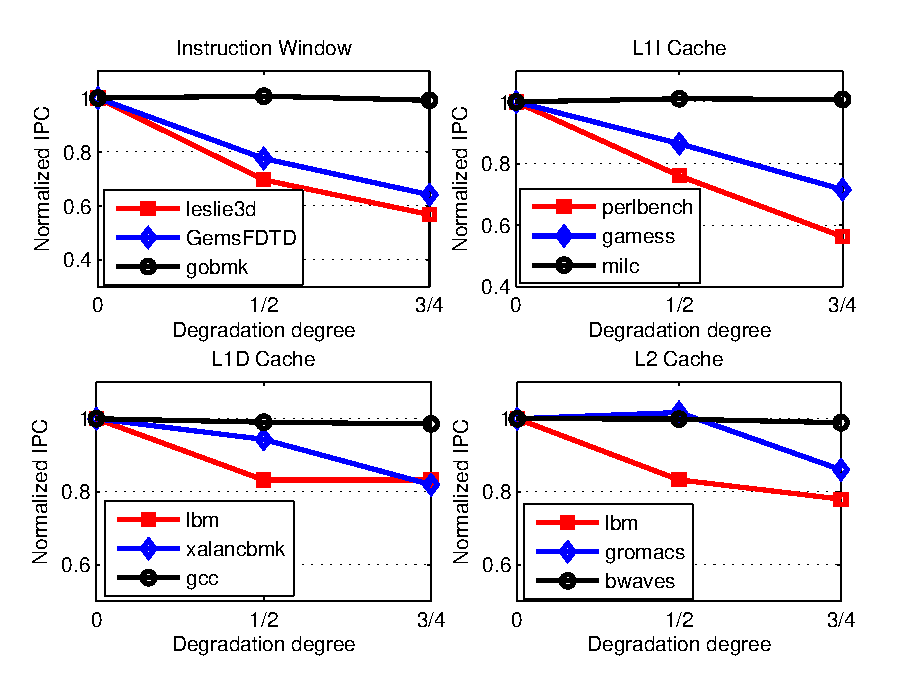
\includegraphics[width=0.75\textwidth]{IPCDegradation.eps}\\
    \caption{Performance degradation  vs. defect degrees of inst. window  (UL), L1 inst. cache (UR), L1 data cache(LL), L2 cache(LR)}
    \label{degrade}
\end{figure}

In the second part of this chapter, we propose a statistical core ranking mechanism, called "CoreRank", to dynamically quantify individual core's healthy condition. CoreRank indicates the OS to avoid the unhealthy cores as much as possible, and always prioritize the healthier ones. Since the healthy condition can be reflected by the performance responses, and quantifying healthy condition is not very timing critical,  we can sample sufficient runtime performance statistics to infer each core's healthy condition. These statistics can be obtained by performance counters. Note that the inference is not one-time procedure, but in a progressive way. CoreRank never finishes its mission even all cores are testified, but periodically invoked to keep tracking them over the lifetime to capture the in field degradations. CoreRank establishes two principles: First, unlike distinguishing between faulty and fault-free cores in the realm of design for reliability, healthy condition should be a "conditional" probability, given a core's healthy condition is highly workload dependent. For example, a core with a faulty branch predictor shows to be healthier when comes to  branch-non-intensive applications than to branch-intensive ones. The application-dependent characteristic implies that the healthy condition should be conditionally defined. Second, CoreRank should not be tied with any specific applications. Quantifying healthy condition towards different applications is less useful because 1) the applications can be extremely diversified, and 2) the impact of inter-application interference on a highly parallel architecture is sporadic and hard to quantify.  CoreRank quantifies healthy condition towards  more specific phase representations, called "snippets", which are dynamic micro-operation streams and oblivious to all of the software level interferences. The snippet can be readily characterized by build-in performance counters, without any instrumentation to running workloads.

\section{Processor Vulnerability Evaluation}
\subsection{Vulnerability Analysis Methods}
Our work is related to several recent researches on characterizing the vulnerability of microprocessor structures to soft errors and hard faults. Architecture vulnerability factor (AVF) is a widely used metric to characterize the masking effect of soft errors both from microarchitecture level and architecture level \cite{mukherjee2003systematic},\cite{biswas2005computing} \cite{fu2006sim}. A structure’s AVF is the probability that a soft error in it causes an external visible error. The AVF can be calculated as the average-over-time percent of architecturally correct execution (ACE) bits in a structure. The ACE bits are those if been changed will affect the final output of a program, and on the contrary, un-ACE bits are those if been changed will not propagate to program output. For example, the AVF of a storage cell is the percentage of cycles the cell contains ACE bits; the AVF of a function unit is the percentage of cycles the unit processes ACE bits or ACE instructions. ACE bit analysis is carried out with a performance level simulator during program execution. Equation \ref{eq:avf} describes how to compute a structure’s AVF through ACE bit analysis, where $B$ is the total bits in a hardware structure, $T$ is the execution cycles of a program, and $N_{ACE}^{t}$ is the number of ACE bits in the structure at a specific cycle $t$.

\begin{equation} \label{eq:avf}
    AVF=\frac{\sum_{t=0}^{T}N_{ACE}^{t}}{B \times T}
\end{equation}


Another method to compute AVF is through statistical fault injection \cite{wang2004characterizing} \cite{touloupis2007study}. Fault injection experiments are performed on a register transfer level (RTL) model of microprocessors. After injecting a fault, the architecture state of the fault injected simulator will be compared with a golden model to determine whether the injected fault results in an external error. After a huge number of fault injections, the percentage of faults leading to external errors is taken as AVF. Statistical fault injection is able to simulate any execution path and allows for high accuracy estimation. Most recently, Walcott et al. \cite{walcott2007dynamic} use linear regression to identify the correlation between AVF and several key performance metrics (such as instructions per cycle and reorder buffer occupancy), and then use the predictive model to compute AVF dynamically during program execution. Duan et al. \cite{duan2009versatile} propose an alternative prediction method to compute AVF across different workloads and microprocessor configurations using boosted regression trees and patient rule induction method.

Prior works also demonstrate that AVF varies significantly and highly depends on microarchitecture structures and architecture programs \cite{pan2009online}. In order to characterize the vulnerability of a program independent of microarchitecture structures, Sridharan et al. \cite{sridharan2009eliminating} propose PVF to evaluate the masking effect of soft errors at architecture level. They use A-bits (like ACE bits) and architecture resources (the structures which can be seen from the perspective of programmers, such as register file and arithmetic logic unit) to compute PVF. Equation \ref{eq:pvf} is utilized to compute an architecture resource’s PVF where $B$ represents the total bits in the architecture resource, $I$ represents the total number of instructions in the program and $N_{A-bit}^{i}$ represents the number of A-bits in instruction $i$. PVF can be used to quantitatively estimate the masking effect of a program to soft errors and to express the behavior of AVF when executing a program. There are also several practical uses of PVF, such as choosing proper algorithms and compiler optimizations to reduce the vulnerability of a program to soft errors. Recently, Sridharan et al. \cite{sridharan2010using} propose another metric HVF to analyze the vulnerability to soft errors only from microarchitecture level.

\begin{equation} \label{eq:pvf}
    PVF=\frac{\sum_{i=0}^{I}N_{A-bit}^{i}}{B \times I}
\end{equation}

AVF, PVF, and HVF, all of them are focusing on the masking effect of soft errors. Bower et al. \cite{bower2006applying} propose a metric named H-AVF for hard faults. H-AVF allows designers to compare alternative hard-fault tolerance schemes. For a given program, a structure’s H-AVF can be computed as Equation \ref{eq:havf} where $N_{i}$ represents the total number of instructions in the program, $N_{f}$ represents the total number of fault sites in the structure, and $inst_{error}$ represents the number of instructions that will be corrupted due to hard faults. The purpose of H-AVF is to evaluate whether a particular sub-structure in microprocessors will benefit from hardening. It can also be used to compare hard-fault tolerance designs thus to provide a quantitative basis for comparison of alternative designs. Besides, Pellegrini et al. \cite{pellegrini2008crashtest} propose a resiliency analysis system called CrashTest. CrashTest is capable of orchestrating and performing a comprehensive design resiliency analysis by examining how the design reacts to faults during program execution. This method mainly considers the impact of hard faults and soft errors on program execution.

\begin{equation} \label{eq:havf}
    H-AVF=\frac{1}{N_{i}} \times \frac{1}{N_{f}} \times \sum_{\forall fault}^{}\sum_{\forall inst}^{}inst_{error}
\end{equation}

Unlike soft errors and hard faults, intermittent faults have many uncertain causes and their behaviors vary significantly. However, the vulnerability of microprocessor structures to intermittent faults is rarely considered. In this paper, we propose a metric IVF to characterize the vulnerability of microprocessor structures to intermittent faults. We compute IVFs for different microprocessor structures considering three intermittent fault models: intermittent stuck-at-1 and stuck-at-0 faults, intermittent open and short faults, and intermittent timing faults.

\subsection{Intermittent Fault Oriented Analysis}
This section first describes our IVF evaluation algorithms for different intermittent fault models, and then presents the equations for IVF computation. A structure’s IVF is defined as the probability that an intermittent fault in the structure leads to an external visible error. The higher IVF, the more a structure is vulnerable to intermittent faults. In modern microprocessors, reorder buffer and register file are two of the most important hardware structures.

\begin{figure}[t]
    \centering
    \includegraphics[width=0.75\textwidth]{IVF-fig4}\\
    \caption{(a) Schematic diagram of a baseline microprocessor. The two gray units are the structures under analyzing; (b) Reorder buffer entry \cite{shen2013modern}}
    \label{fig:baseline-processor}
\end{figure}


Fig. \ref{fig:baseline-processor}(a) shows a baseline pipeline used in this work. Reorder buffer is used for out-of-order instruction execution, which allows instructions to be committed in-order. It keeps the information of in-flight instructions and allows for precise exceptions and easy rollback for control of target address mispredictions. The entry in reorder buffer is allocated in a round-robin order. Fig. \ref{fig:baseline-processor}(b) further shows typical fields contained in an entry of reorder buffer \cite{shen2013modern}. These fields have different functions. The busy flag, issued flag, finished flag, speculative flag, and valid flag are control signals, while $PC$ denotes the address of the current instruction, and rename register shows the renamed register for the destination register of an instruction. For register file, it is an array of processor registers and will be used to provide operation data during program execution. Each register in it contains 64 bits. If any of these two structures is affected by an intermittent fault, the probability resulting in a visible error is very high.We compute IVFs for these two representative structures in this work.

Before IVF computation, the following two questions should be carefully answered.

1) How to determine whether an intermittent fault affects program execution?

2) In order to describe intermittent faults, how to set these three key parameters: burst length, active time, and inactive time appropriately?

For the first question, to evaluate the impact of an intermittent fault on program execution, we need to determine whether the fault propagates to a storage cell and changes ACE bits during its lifetime. For intermittent stuck-at faults, as they only affect a single location, we should check whether the affected location contains an ACE bit, and then analyze whether the ACE bit is upset during the fault’s active time. Only the case when the affected location contains an ACE bit and the ACE bit is changed will affect program execution. For intermittent open and short faults, they may corrupt two adjacent bit lines. When such a fault occurs, we need to determine whether the fault propagates to a storage cell and change ACE bits. While for intermittent timing faults, they may cause timing violations and affect write operations. Only when an intermittent timing fault has been captured by a storage structure and changes ACE bits, it will affect program execution.

\begin{figure}[t]
    \centering
    \includegraphics[width=0.75\textwidth]{IVF-fig5}\\
    \caption{Example of intermittent timing faults caused by voltage emergencies.}
    \label{fig:timing-faults}
\end{figure}

For the second question, the parameters of an intermittent fault should follow the characteristics of an actual fault. As intermittent faults may be caused by different factors, the duration of intermittent faults could vary across a wide range of timescale. To set appropriate values for these key parameters, we analyze one kind of intermittent timing faults caused by significant voltage variation. The situation when supply voltage variation across a allowed voltage threshold is called a voltage emergency \cite{joseph2003control}. Voltage emergencies will lead to timing violations by slowing logic circuits. Fig. \ref{fig:timing-faults} shows an example of intermittent timing faults caused by voltage emergencies. As can be seen, intermittent timing faults caused by voltage variations usually last on the order of several to tens of nanoseconds. Prior works also show the similar duration of an intermittent fault \cite{smolens2007detecting} \cite{gracia2008analysis} \cite{stathis2001physical}. According to the observation, we set the burst length of an intermittent fault in the range of 5 cycles to 30 cycles in our experiments. Both active time and inactive time are set to 2 cycles. The number of activations will be changed according to burst length, but the 50\% duty cycle is kept constant. For an instance, if burst length is 30-cycle, the number of activations is 8. Besides, as the appearance time of intermittent faults cannot be predicted, their start time are randomly generated during program execution.

Based on the above analysis, the first step for IVF computing is to determine ACE bits in a structure during program execution; the second step is to check whether ACE bits are changed when an intermittent fault occurs. As reorder buffer is used to support out-of-order instruction execution, we analyze ACE bits in it by monitoring instructions when these instructions go through all stages of the pipeline. Meanwhile, register file is used to store and provide operation data for in-flight instructions, we analyze ACE bits in it based on its related operations, such as read, write, and evict. Following we present IVF computation algorithms for intermittent stuck-at faults, intermittent open and short faults, and intermittent timing faults, respectively.

\subsubsection{Intermittent Stuck-at Faults}
Intermittent stuck-at faults include intermittent stuck-at-1 faults and intermittent stuck-at-0 faults. As the analysis methods for these two kinds of faults are similar, for the sake of brevity, we take intermittent stuck-at-1 faults as an example in this section.

\begin{figure}[t]
    \centering
    \includegraphics[width=0.75\textwidth]{IVF-fig6}\\
    \caption{ACE bits and un-ACE bits projection for IVF computing.}
    \label{fig:ACEbits}
\end{figure}

1) Reorder Buffer: We illustrate the IVF computation algorithm for reorder buffer at first. Unlike a soft error only existing for a single cycle, an intermittent fault will last for a while and repeatedly appear during its lifetime. Fig. \ref{fig:ACEbits} shows a 3-D perspective of a simplified reorder buffer. The X-axis represents the number of entries in the structure, the Y-axis represents the number of bits in each entry, and the Z-axis represents the time of program execution. For the example structure, it has two entries and each entry contains two bits. The small black parallelograms and white parallelograms are used to indicate ACE bits and un-ACE bit, respectively. For this example, we assume an intermittent stuck-at-1 fault occurs. The burst length is set to 2 cycles, while both active time and inactive time are 1 cycle.

The gray part of the cube shows the possible affected region by the fault. The parallelograms in the X-Y plane are planar representation of ACE bits and un-ACE bits for the gray part. For a specific bit, if it contains an ACE bit during the fault’s active time and its value is changed by the fault, the projection of that bit in X-Y plane is an ACE bit, otherwise, the projection will be an un-ACE bit. As can be seen in Fig. \ref{fig:ACEbits}, during the fault’s active time, $B_1$ and $B_2$ contain ACE bits and will be affected by the fault. Though $B_1$ and $B_3$ contain ACE bits in the fault’s inactive time, they will not be affected by the fault. To generate bit projection, we further need to analyze whether the values in and will be changed. For the intermittent stuck-at-1 fault, only if an ACE bit is supposed to be a logic value “0”, it will actually be corrupted. Fig. \ref{fig:ACEbits} shows the values of $B_1$ and $B_2$ during the active time. As the fault in-question is an intermittent stuck-at-1 fault, only the projection of $B_1$ is an ACE bit and other three bits are un-ACE bits. In this case, the probability that the fault leads to an external visible error is 25\%, which means the IVF is 25\%. With the above ACE bit analysis and bit projection, we can quickly determine whether an intermittent stuck-at fault affects program execution and further compute IVF for reorder buffer.

\begin{figure}[t]
    \centering
    \includegraphics[width=0.75\textwidth]{IVF-fig7}\\
    \caption{Lifetime of a register version with related operations. $F_1$, $F_2$, and $F_3$ are three intermittent stuck-at faults occurring at different time.}
    \label{fig:register-lifetime}
\end{figure}


2) Register File: Unlike reorder buffer, the ACE bits analysis for register file is a little different. The ACE bits in register file are analyzed according to the related operations on each physical register. During the execution of a program, if the microprocessor decodes an in-flight instruction with a destination register, it will allocate a free physical register for the instruction, creating a new register version \cite{montesinos2007using}. The lifetime of a register version is shown in Fig. \ref{fig:register-lifetime}. During the lifetime of a register version, the possible operations include allocation ($A$), write ($W$), read ($R$), and deallocation ($D$). A register version can only be written once but can be read several times during its lifetime. The lifetime of a register version is from allocation to deallocation and can be divided into three intervals: from allocation to write ($A$ to $W$), from write to the last read ($W$ to $R_n$), and from the last read to deallocation ($R_n$ to $D$). Only the interval from write to the last read is critical time and other two intervals belong to noncritical time. During the critical time, all bits in the register are ACE bits.

If an intermittent stuck-at-1 fault occurs during the critical time, these ACE bits with logic value “0” will be affected and lead to an external visible error (like fault $F_1$). If the fault occurs during noncritical time, it will always be masked (like fault $F_3$). A complicated situation is that a fault may start from a critical time region and end at a noncritical time region (like fault $F_2$). For this kind of fault, if its residency time in critical time region overlaps its active time, the fault can be handled like $F_1$; if there is no overlap, the fault will be masked. Only when an intermittent stuck-at-1 fault occurs during critical time and changes ACE bits will affect program execution. With the above analysis, the IVF for reorder buffer and register file considering intermittent stuck-at faults can be expressed as Equation. \ref{eq:IVF-SA} where $B$ represents the total number of bits in the structure under analysis, $s$ represents a location in the structure, $D$ represents the burst length of an intermittent stuck-at fault, and $U_{ACE}^D(s)$ represents whether an ACE bit in location will be changed by the fault; if it is, the value is assigned to one; otherwise, the value is assigned to zero. The numerator adds the total number of ACE bits that will be affected during the lifetime of an intermittent stuck-at fault.

\begin{equation} \label{eq:IVF-SA}
    IVF_{sa}=\frac{\sum_{s=1}^{B}U_{ACE}^{D}(s)}{B}
\end{equation}

\subsubsection{Intermittent Open and Short Faults}
Intermittent open and short faults have different behaviors depending on where they occur. They also can be taken as intermittent stuck-at faults or intermittent timing faults for some cases. Intermittent bridging faults, one kind of intermittent short fault, are different from intermittent stuck-at faults and intermittent timing faults. Intermittent bridging faults describe the cases when two signal wires are shorted together. They can be divided into four types: wired-AND, wired-OR, dominant-AND, and dominant-OR. For intermittent wired bridging faults, the logic value of the shorted nets is modeled as a logical AND or OR of the logic values on the shorted wires, while for intermittent dominant bridging faults, one wire is modeled to dominate the logic value on the shorted nets. The wired bridging faults were originally developed for bipolar circuits, while dominant bridging faults were for CMOS devices. Since CMOS technology is widely used for microprocessor manufacturing, we only analyze the dominant bridging faults in this work. An intermittent dominant bridging fault will corrupt two adjacent bit lines which produce two-bit of corruption.

\begin{figure}[t]
    \centering
    \includegraphics[width=0.75\textwidth]{IVF-fig8}\\
    \caption{Intermittent dominant-AND and dominant-OR bridging faults (a) in reorder buffer and (b) in register file.}
    \label{fig:IM-AND-OR}
\end{figure}


Fig. \ref{fig:IM-AND-OR}(a) and (b) show intermittent dominant-AND and dominant-OR bridging faults in the metal interconnect wires to reorder buffer and register file, respectively. and are aggressor wires, while and are victim wires. The logic value of the victim wire is dominated by the AND operation or OR operation of the logic value of the aggressor wire and its own value. For intermittent dominant-AND and dominant-OR faults, their controlling values are logic value “0” and logic value “1”, respectively. These two kinds of faults also have similar analysis methods, for the sake of brevity, we only take dominant-AND bridging faults as an example. The intermittent open and short faults refer to intermittent dominant-AND bridging faults if not specifically mentioned in the following analysis. When an intermittent dominant-AND bridging fault occurs, the value of the victim wire will be changed only when the victim wire has a logic value “1” and the aggressor wire has a logic value “0”. The corrupted data of the victim wire then propagates during program execution. If the corrupt data propagates to a storage cell, we further need to determine whether the affected bit is an ACE bit or not. If it is an ACE bit, then the fault will result in an external visible error; otherwise, the fault is said to be masked. 

To compute IVFs of reorder buffer and register file for intermittent dominant bridging faults, we also need to analyze the data fields in them. As can be seen in Fig. \ref{fig:IM-AND-OR}(a), if the control bit in a reorder buffer entry has been corrupted, the instruction will be in a wrong state, and may lead to a fatal error. If the destination register tag is affected, the instruction result will be written to a wrong register. The bits in a register [shown in Fig. \ref{fig:IM-AND-OR}(b)], however, make no difference to the data if been affected, there is no need to further differentiate them.We only check the value containing in two adjacent lines and determine whether the fault changes ACE bits in that register. 

With the above analysis, the IVF for reorder buffer and register file considering intermittent dominant bridging faults can be expressed as Equation \ref{eq:IVF-BF} where $NUM$ represents the total number of intermittent dominant bridging faults, $P_{ACE}^{e}$ represents whether a fault $e$ propagates to reorder buffer or register file and finally affects ACE bits. If true, $P_{ACE}^{e}$ will set to one. Otherwise, $P_{ACE}^{e}$ will set to zero and the fault is said to be masked.

\begin{equation} \label{eq:IVF-BF}
    IVF_{bf}=\frac{\sum_{e=1}^{NUM}P_{ACE}^{e}}{NUM}
\end{equation}

\subsubsection{Intermittent Timing Faults}
Unlike intermittent stuck-at faults which transform the correct value to a constant value, intermittent timing faults will affect data propagation and leads to capture wrong data to storage structure at entry level.

\begin{figure}[t]
    \centering
    \includegraphics[width=0.75\textwidth]{IVF-fig9}\\
    \caption{Intermittent timing fault results in writing a wrong data to a storage cell.}
    \label{fig:IM-timing-fault}
\end{figure}

Before presenting the algorithm to compute IVF for intermittent timing faults, we need to know when a fault will affect program execution. To determine the impact of an intermittent timing fault, two steps are needed. First, analyze whether the fault is captured by a storage cell; second, check whether ACE bits in the storage cell have been affected. Only when an intermittent timing fault propagates to storage cells and changes ACE bits, it will affect the final program output. Otherwise, the fault will not manifest itself in external output and is said to be masked. In this work, we assume an intermittent timing fault only cause timing violations during its active time. If a write operation occurs during the active time of an intermittent timing fault, we assume the fault propagates to the structure. If no write operations occur or write operations only occur during inactive time, the fault is said to be masked and will not affect program execution. We use an example to further explain for this. Fig. \ref{fig:IM-timing-fault} illustrates whether an intermittent timing fault will lead to capture a wrong data to a storage cell. As can be seen, write operation $W_1$ occurs during the active time of $Fault_1$, the fault will propagate to a storage cell. While write operation $W_2$ occurs during the inactive time of $Fault_2$, the fault will not affect the data propagation.

With the above analysis, the frequency of write operations has strong correlation with the vulnerability of a structure to intermittent timing faults. During the lifetime of an intermittent timing fault, a structure with high write frequency is more vulnerable because the probability a fault propagating to the structure is very high. On the contrary, a structure with low write frequency is less vulnerable. To compute the IVF for different structures, we then need to determine whether a write operation is taken during the active time of an intermittent timing fault. For reorder buffer, the related write operations occur when the state of an instruction in it changes. For register file, the related write operations take place when an instruction commits or when a value is loaded from memory. The related write operations will be recorded for IVF computation during program execution.

When a wrong data has been captured by a structure, we need to further analyze whether ACE bits in that cell have been changed by the fault. If ACE bits are upset, the fault will affect the external visible output. Otherwise, it is said to be masked at architecture level. There are mainly two scenarios that an intermittent timing fault will be masked during program execution: first, the data in a storage structure is proved to be a dead value; second, the captured data only changes un-ACE bits. If an intermittent timing fault is in either of the two scenarios, it will not affect program execution. Which scenario occurs is determined by analyzing ACE bits and un-ACE bits in different structures. For example, Fahs et al. \cite{fahs2001performance} found that about 14\% instructions are dead instructions during executing SPEC CPU2000 benchmarks. Dead instructions are those instructions whose results will not be used by any other instructions in the future. If the result of a dead instruction is changed by an intermittent timing fault, even if an incorrect data has been written to register file, the fault will not affect program execution. By analyzing ACE bits and un-ACE bits in different structures during program execution, we can determine which scenario occurs.

Only an intermittent timing fault propagates to a storage cell and changes ACE bits, it will contribute to IVF computation. The IVF considering intermittent timing faults can be expressed as Equation \ref{eq:IVF-TF} where $NUM$ represents the total number of intermittent timing faults during executing a program; $P_{NUM}$ represents the number of intermittent timing faults propagating to the structure; $N_{dead}$ represents the number of faults only affecting dead values; $N_{un-ACE}$represents the number of faults only changing un-ACE bits. With this equation, we can compute $IVF_{tf}$ for different microprocessor structures.

\begin{equation} \label{eq:IVF-TF}
    IVF_{tf}=\frac{P_{NUM}-(N_{dead} + N_{un-ACE})}{NUM}
\end{equation}

\subsubsection{Statistical Significance}
In this work, we use statistical sampling to study the characteristics of intermittent faults. To make the evaluation having statistical significance, a large number of faults should be analyzed during a simulation. After trying different number of faults, we set the fault number as 1000 to make a tradeoff between accuracy and analysis time. Besides, the burst length and the number of activations in an intermittent fault have significant impact on IVF computation. During executing different benchmarks, the two parameters will be changed to make our analysis more comprehensive, and the final IVF of a structure is the average result across all faults under analysis.

With the above introduced (5)–(7), we can quickly compute IVFs for reorder buffer and register file. Furthermore, our proposed IVF estimation methodology also can be extended to other structures, such as issue queue, load/store queue, and L1/L2 caches. As the analysis of ACE bit in issue queue and load/store queue is also based on tracking the ACE bits in instructions when these instructions go through the pipeline, which is similar to the ACE analysis of reorder buffer. Besides, the analysis of ACE bit in L1/L2 caches is based on dividing the lifetime of a data block into critical time and noncritical time, which is similar to the ACE analysis of register file. Therefore, our IVF estimation methodology is also suitable for these structures. As all the above mentioned storage structures may occupy more than 60\% area of modern microprocessors \cite{Itanium_isscc08}, our proposed evaluation methodology provides a generic metric for reliability estimation.

\subsection{Experiment Result Analysis}
\subsubsection{Experiment Setups}
All of our experiments are conducted on the Sim-Alpha simulator \cite{desikan2001sim}. Sim-Alpha is a validated execution-driven simu-lator for Alpha 21264 microprocessor \cite{skessler1999alpha}. It can execute instructions down the mis-speculated path, in the same way as an actual microprocessor would execute them. In this work, Sim-Alpha is heavily modified to support IVF computing for reorder buffer and register file. We use all the twelve SPEC CPU2000 integer benchmarks to evaluate our method. Since the simulator cannot accurately simulate the floating-point pipeline, the floating-point benchmarks are not included in our experiments. All the benchmarks are compiled for the Alpha ISA. In order to reduce simulation time, we use Simpoint tool \cite{sherwood2002automatically} to pick the most representative simulation point for each benchmark and each benchmark is fast-forwarded to its representative point before detailed performance simulation takes place. Each benchmark is evaluated for 100 million instructions using the full reference input set. The baseline configuration of the simulator is further summarized in Table \ref{tab:sim-config}. As we focus on the integer pipeline, only the integer pipeline resources are shown in the table. Besides, to analyze the impact of different microarchitecture design parameters on IVF computation, we further change the number of fetch/slot/issue width, commit width, reorder buffer size, and register file size in our experiments.

\begin{table} 
    \centering
    \caption{Simulated Microprocessor Configuration}
    \begin{tabular}{@{}l|l@{}}
        \toprule
        Configuration Parameter & Value \\ \midrule
        Pipeline Stages & 7 \\
        Fetch/Slot/Issue/Commit Width & 4/4/4/11 instruction/cycle \\
        Branch-Predictor Type & Hybrid, 4K global + 2-level 1K local + 4K choice \\
        Integer Register File Size & 80 entries  \\
        Integer Issue Queue Size & 20 entries \\
        Reorder Buffer Size & 80 entries \\
        Unified Load/Store Queue Size & 64 entries \\
        Integer ALUs & 4, 1-cycle latency \\
        Integer Multipliers/Dividers &  \\
        L1 Data Cache & 64KB, 2-way, 64 byte line-size, 1-cycle latency \\
        L1 Instruction Cache & 64KB, 2-way, 64 byte line-size, 3-cycle latency \\
        L2 Unified Cache & 2MB, direct mapped, 64 byte line-size, 7-cycle latency \\
        I-TLB/D-TLB & 128-entry, full-associative \\ \bottomrule
    \end{tabular}
    \label{tab:sim-config}
\end{table}

\subsubsection{IVF Computation for Different Intermittent Fault Models}
we first present IVF of reorder buffer and register file considering different intermittent fault models, and then compute IVF by changing microarchitecture parameters and program phases. Finally, we introduce several IVF guided protection techniques to improve system reliability. In our experiments, we compute IVF with different fault configurations by changing the key parameters of intermittent faults. The burst length of each intermittent fault is assigned to 6 cycles, 10 cycles, and 22 cycles, respectively. Both active time and inactive time are assigned to 2 cycles. The start time of each intermittent fault is randomly generated during program execution.

\begin{figure}[t]
    \centering
    \includegraphics[width=0.95\textwidth]{IVF-fig10}\\
    \caption{Reorder buffer (left part) and register file (right part) AVFs considering soft errors and $IVF_{sa1}$ considering intermittent stuck-at-1 faults.}
    \label{fig:AVF-sa1}
\end{figure}

\begin{figure}[t]
    \centering
    \includegraphics[width=0.95\textwidth]{IVF-fig11}\\
    \caption{Reorder buffer (left part) and register file (right part) $IVF_{sa0}$ considering intermittent stuck-at-0 faults.}
    \label{fig:AVF-sa0}
\end{figure}


1) Intermittent Stuck-at Faults: For intermittent stuck-at faults, as the value of ACE bits will affect IVF evaluation, we compute $IVF_{sa1}$ in terms of intermittent stuck-at-1 fault model and $IVF_{sa0}$ in terms of intermittent stuck-at-0 fault model, respectively.

Fig. \ref{fig:AVF-sa1} and Fig. \ref{fig:AVF-sa0} show $IVF_{sa1}$ and $IVF_{sa0}$ for reorder buffer and register file during executing different benchmarks. The average $IVF_{sa1}$ for reorder buffer and register file vary from 21\%  to 37\% and from 21.4\% to 31.5\%, respectively. The average $IVF_{sa0}$, however, vary from 5.8\% to 10.3\% and from 1.1\% to 1.6\%, respectively. As can be seen, the longer burst length, the more ACE bits been affected, which leads to a higher $IVF_{sa1}$ and $IVF_{sa0}$. For a same burst length, the average $IVF_{sa1}$ is much higher than $IVF_{sa0}$. This is because during executing different benchmarks, the number of ACE bits containing logic value “0” is much more than these containing logic value “1”, especially in register file. ACE bits with logic value “0’ are vulnerable to intermittent stuck-at-1 faults, but not to intermittent stuck-at-0 faults. Meanwhile, both $IVF_{sa1}$ and $IVF_{sa0}$ of reorder buffer are much higher than that of register file. The reason is that the residency time of an instruction in reorder buffer is very long, from issue stage till commit stage. Register file, however, will be written very frequently, making its vulnerable time much shorter than that of reorder buffer.

We also present the AVFs of reorder buffer and register file considering soft errors in Fig. \ref{fig:AVF-sa1}. Compared to $IVF_{sa1}$, their AVFs are much lower. As an intermittent stuck-at-1 fault has longer duration than soft errors and most ACE bits contain logic value “0” in the two structures, which makes the probability an intermittent stuck-at-1 fault affecting final program execution is much higher. Therefore, intermittent stuck-at-1 faults have much more serious impact on program execution than soft errors if occur. The situation for intermittent stuck-at-0 faults, however, is just on the contrary. The reason is that soft errors can flip all the ACE bits while intermittent stuck-at-0 faults only affect these ACE bits with logic value “1”. 

\begin{figure}[t]
    \centering
    \includegraphics[width=0.95\textwidth]{IVF-fig12}\\
    \caption{$IVF_{bf}$ for reorder buffer (left part) and register file (right part) considering intermittent dominant-AND bridging faults.}
    \label{fig:IVF-and}
\end{figure}

2) Intermittent Open and Short Faults: Fig. \ref{fig:IVF-and} shows $IVF_{bf}$ for reorder buffer and register file considering intermittent dominant-AND bridging faults. As can be seen, for different burst length, the average $IVF_{bf}$ for reorder buffer and register file vary from 14.8\% to 23\% and from 11.5\% to 22.8\%, respectively. These two structures have relatively low vulnerability to inter-mittent dominant bridging faults. When an intermittent dominant bridging fault occurs, only the case that the aggressor wire holds a controlling value and the victim wire holds a non-controlling value, the fault can propagate during program execution. With the same burst length, reorder buffer has a little higher than that for register file. The explanation is as follows: for reorder buffer, the control bits are more sensitive to intermittent dominant bridging faults; while for register file, however, it contains many narrowvalues during program execution. A value is categorized as narrow only if its leading bits are all zeros or ones. Kumar et al. \cite{kumar2006reducing} show about 50\% of the produced results could be categorized as narrow values. For the narrow values in register file, they have higher masking rates to intermittent dominant bridging faults, which results in a lower $IVF_{bf}$.

\begin{figure}[t]
    \centering
    \includegraphics[width=0.95\textwidth]{IVF-fig13}\\
    \caption{$IVF_{tf}$ for reorder buffer (left part) and register file (right part) considering intermittent faults.}
    \label{fig:IVF-tf}
\end{figure}


3) Intermittent Timing Faults: We further present $IVF_{tf}$ results for reorder buffer and register file considering intermittent timing faults. Fig. \ref{fig:IVF-tf} shows the $IVF_{tf}$ for reorder buffer and register file during executing different benchmarks. As can be seen, the average $IVF_{tf}$ for reorder buffer and register file are from 15.8\% to 23.7\% and from 19.7\% to 30.6\%, respectively. The longer burst length, the more write operations will be affected, which leads to higher $IVF_{tf}$ results. From Fig. \ref{fig:IVF-tf}, we can tell that the average $IVF_{tf}$ of register file is a little higher than that of reorder buffer, this is because register file provides operands for each instruction and has higher write frequency than reorder buffer. There is also a notable exception during executing two benchmarks gap and gzip. As for these two benchmarks, they have much higher cache miss rates than other benchmarks. During the time a cache miss occurs, the write operation for reorder buffer and register file will reduce dramatically, which leads to a much lower $IVF_{tf}$ at that time. The widely used method to tolerate timing violations is to set a wider timing margin \cite{annavaram2007implications}. Only the intermittent timing faults occurring at critical paths and resulting in timing margin violation are what need to be considered.

4) Comparisons: Figs. \ref{fig:AVF-sa1}, Fig. \ref{fig:IVF-and}, and Fig. \ref{fig:IVF-tf} have shown IVFs of reorder buffer and register file for three intermittent fault models. We then give a comparison of the impact of these faults. From these figures, it is easy to tell that intermittent stuck-at-1 faults have most serious impact on program execution during executing most benchmarks. For all these fault models, when the burst length of an intermittent fault increases, the probability to cause external errors is also increase, which means a structure’s IVF will increase. Besides, for a same fault model, the IVFs of reorder buffer and register file also vary significantly. Reorder buffer is more sensitive than register file to intermittent stuck-at faults and intermittent open and short faults, while less sensitive to intermittent timing faults. Utilizing the proposed IVF evaluation methodology, designers can quantitatively analyze the masking effect of intermittent faults and guide system reliability design during the early design stage.

In this work, we focus on the impact of intermittent faults, while Pellegrini et al.’s work CrashTest \cite{pellegrini2008crashtest} analyzes the impact of hard faults and soft errors on program execution. Their experimental results shows that about 80\% of stuck-at faults will cause errors, while only 40\% of path-delay faults have adverse effects on program execution. Soft errors have the least impact on the correct functionally of the design and on average less than 10\% of them cause an error. Comparing their results with our experimental results, it is easy to knowthat hard faults have most serious impact on program execution, followed by intermittent faults, and finally soft errors. Pellegrini et al.’s work combined with our work provides a global reliability picture for designers to understand the impact of different kinds of faults on program execution.

\subsubsection{IVF Computation for Different Microprocessor Configurations and Program Phases}
We have computed IVF for different intermittent fault models under a specified microprocessor configuration. In this subsection, we further extend our proposed methodology to address different microprocessor configurations. We choose four microarchitecture design parameters (fetch/slot/issue width, commit width, reorder buffer size, and register file size) which are believed to have impact on IVF computation. We change the size of these parameters to generate different microprocessor configurations. Table \ref{tab:ROB-config} and Table \ref{tab:RF-config} show four different microprocessor configurations for reorder buffer and register file, respectively. Of these configurations, rob\_base and reg\_base are the baseline configurations. We compute reorder buffer’s and register file’s IVF for each configuration shown in Table \ref{tab:ROB-config} and Table \ref{tab:RF-config}. Burst length is set to 10 cycles in the following experiments.

\begin{table}
    \caption{Different Microprocessor Configurations for Computing IVF of Reorder Buffer}
    \begin{tabular}{c|cccc}
        \hline
        & Fetch/Slot/Issue Width & Commit Width & Reorder Buffer Size & Simulated Workloads   \\ \hline
        rob\_base & 4 & 11 & 80 & \multirow{4}{*}{All twelve SPEC CPU2000 integer benchmarks} \\
        rob\_c1 & 4 & 11 & 40 & \\
        rob\_c2 & 4 & 11 & 120 & \\
        rob\_c3 & 2 & 5 & 80 & \\ \hline
    \end{tabular}
    \label{tab:ROB-config}
\end{table}

\begin{table}
    \caption{Different Microprocessor Configurations for Computing IVF of Register File}
    \begin{tabular}{c|cccc}
        \hline
         & Fetch/Slot/Issue Width & Commit Width & Register File Size & Simulated Workloads \\ \hline
         reg\_base & 4 & 11 & 80 & \multirow{4}{*}{All twelve SPEC CPU2000 integer benchmarks} \\
         reg\_c1 & 4 & 11 & 60 &  \\
         reg\_c2 & 4 & 11 & 120 & \\
         reg\_c3 & 2 & 5 & 80 & \\ \hline
    \end{tabular}
    \label{tab:RF-config}
\end{table}


Fig. \ref{fig:ROB-IVF-base}, Fig. \ref{fig:ROB-IVF-C1}, Fig. \ref{fig:ROB-IVF-C2}, and Fig. \ref{fig:ROB-IVF-C3} present our computed IVF results for different intermittent fault models. Each figure represents the result for one configuration. As can be seen, for configurations rob\_c1 and reg\_c1, reorder buffer’s and register file’s IVFs are much higher than the results of the baseline configuration. That is because when reduce a structure’s size, its occupancy increases greatly and the structure will be more vulnerable to intermittent faults. For configurations rob\_c2 and reg\_c2, on the contrary, the occupancy of a structure will reduce, which results in IVF reduction. While for configurations rob\_c3 and reg\_c3, though we reduce instruction fetch width and commit width, their IVFs also decrease significantly. This is due to both the number of in-flight instructions and the number of ACE bits in the pipeline reduces sharply during program execution. The experimental results reflect that a structure’s IVF varies across different microprocessor configurations and has high correlation with its size and the number of in-flight instructions. Besides, we can tell that intermittent stuck-at-1 faults have most serious impact while intermittent stuck-at-0 faults have minimal impact on program execution for most benchmarks. Our proposed IVF evaluation methodology can be easily extended to evaluate IVF for different microprocessor configurations and can be used to choose appropriate microarchitecture parameters during the early design stage.

\begin{figure}[t]
    \centering
    \includegraphics[width=0.95\textwidth]{IVF-fig14}\\
    \caption{Reorder buffer's IVF on configuration rob\_base (left) and register file's IVF on configuration reg\_base (right).}
    \label{fig:ROB-IVF-base}
\end{figure}

\begin{figure}[t]
    \centering
    \includegraphics[width=0.95\textwidth]{IVF-fig15}\\
    \caption{Reorder buffer's IVF on configuration rob\_c1(left) and register file's IVF on configuration reg\_c1(right).}
    \label{fig:ROB-IVF-C1}
\end{figure}


\begin{figure}[t]
    \centering
    \includegraphics[width=0.95\textwidth]{IVF-fig16}\\
    \caption{Reorder buffer's IVF on configuration rob\_c2 (left) and register file's IVF on configuration reg\_c2 (right).}
    \label{fig:ROB-IVF-C2}
\end{figure}

\begin{figure}[t]
    \centering
    \includegraphics[width=0.95\textwidth]{IVF-fig17}\\
    \caption{Reorder buffer's IVF on configuration rob\_c3 (left) and register file's IVF on configuration reg\_c3(right).}
    \label{fig:ROB-IVF-C3}
\end{figure}

Furthermore, we compute $IVF_{sa1}$ of reorder buffer and register file for different program phases. All program phases are chose by Simpoint \cite{sherwood2002automatically} and each contains 1 million instructions. Fig. \ref{fig:ROB-IVF-sa1} and Fig. \ref{fig:RF-IVF-sa1} show $IVF_{sa1}$ of reorder buffer and register file during executing several benchmarks. As can be seen, IVF varies significantly across different program phases and is heavily depended on the characteristics of a program. This phenomenon can be exploited to select proper protection techniques during program execution. We can use heavier protection (strict redundant multithreading) during highly vulnerable phases and lighter protection (partial or no redundant multithreading) during less vulnerable phases. With the dynamic tuning of protection, designers can achieve system reliability while minimize performance and/or energy overhead. The dynamic tuning of protection scheme also has been exploited to protect microprocessors from soft errors \cite{walcott2007dynamic}.

\begin{figure}[t]
    \centering
    \includegraphics[width=0.75\textwidth]{IVF-fig18}\\
    \caption{$IVF_{sa1}$ of reorder buffer for different program phases during executing twolf, vortex, and eon.}
    \label{fig:ROB-IVF-sa1}
\end{figure}

\begin{figure}[t]
    \centering
    \includegraphics[width=0.75\textwidth]{IVF-fig19}\\
    \caption{$IVF_{sa1}$ of register file for different program phases during executing mcf, crafty, and parser.}
    \label{fig:RF-IVF-sa1}
\end{figure}


\subsubsection{IVF Guided Reliable Design}
Our experimental results show that IVFs of reorder buffer and register file varies significantly, implying that these structures have different vulnerability to intermittent faults. Designers can exploit IVF information to determine which parts in microprocessors are most cost-effective to protect. For those structures with high IVFs, some heavyweight protection techniques are needed. We further introduce several possible techniques to improve system reliability.

For intermittent stuck-at faults or intermittent open and short faults, a feasible protection scheme is to harden these high IVF structures with fault detection techniques (such as ECC or parity code). As intermittent faults occur in burst at the same location, if a fault in a storage cell has been detected for a predefined times, we can deduce that an intermittent fault has happened. At that time, a flag bit in the entry will be set to busy, and the entry will be unused for a while to avoid the influence of the intermittent fault. After then, the entry can be used again when the intermittent fault disappears, for example, when the power delivery sub-system returns to its steady-state voltage. The partial protection technique ParShield proposed in \cite{montesinos2007using} also can be used to protect register file from intermittent faults. Meanwhile, for intermittent timing faults, a prior proposed technique Razor \cite{Dan_Micro03} can be combined to these storage cells in critical paths of the most vulnerable structures, for example, Razor can be used to protect architecture registers as they are more vulnerable to intermittent timing faults. Besides, we can exploit architecture level masking of intermittent timing faults to improve system reliability \cite{pan2011cost}.

The above introduced techniques seek to tolerate intermittent faults at fine-granularity. A coarse-granularity technique can be used to deal with intermittent faults in nowadays multi-core or many-core microprocessors. With inherent redundancy in these microprocessors, if a core sustains an intermittent fault, it should be suspended for a period of time, or operating system should transfer threads executing in the faulty core to other spare cores. Once the intermittent fault disappears later, the affected core can be used again.

Besides, we also show that a structure’s IVF varies across different microprocessor configurations and program phases. This phenomenon can be exploited to select microarchitecture design parameters and tune protection schemes online. With the guide of IVF, designers can select appropriate protection techniques for these most vulnerable structures or program phases, which satisfies system reliability design goal while minimize implementation overheads. Nevertheless, combining our IVF evaluation methodology with these protection techniques is beyond the scope of this paper, we plan to exploit protection techniques to detect and recover from intermittent faults in our future work.

\subsection{Discussion}
Intermittent faults are emerging as a big challenge to reliable microprocessor design. In this paper,we propose a metric IVF to quantitatively characterize the vulnerability of microprocessor structures to intermittent faults. The IVF evaluation methodology contains the following aspects:
\begin{itemize}
    \item analyze the physical causes of intermittent faults;
    \item classify intermittent faults into different fault models based on their behaviors;
    \item set key parameters for an intermittent fault and determine when the intermittent fault results in a visible error;
    \item for a specific microprocessor structure, propose IVF computation algorithms for different intermittent fault models;
    \item implement IVF computation algorithms in a high-level performance simulator, with which to compute IVF for the specific structure.
\end{itemize}

With the IVF evaluation methodology, we compute IVFs for reorder buffer and register file in terms of intermittent stuck-at faults, intermittent open and short faults, and intermittent timing faults. Experimental results show that intermittent stuck-at-1 faults have most serious adverse impact on program execution among these three types of intermittent faults. Besides, IVF varies noticeably across different microprocessor structures and program phases. Our experimental results imply partial protection of the most vulnerable structures and program phases to enhance system reliability. With the guide of IVF evaluation methodology, we also discuss several possible intermittent fault detection and recovery techniques which can be used to improve system reliability.

\section{Multi-Core Processor Salvaging}
According to recent ITRS report, reliability issue due to progressive aging mechanism has notched one of the top five near-term (by 2020) challenges  \cite{itrs13}. These aging mechanisms, such as TDDB (Time-Dependent Dielectric Breakdown), NBTI (Negative Bias Temperature Instability), PBTI (Positive Bias Temperature Instability), HCI (Hot-Carrier Injection), RTN (Random Telegraph Noise),  can cause processor degradations, and are blamed for "Sick Silicon". The circuit-level impact can be measured by aging sensors \cite{siliconodometer} \cite{svfdtvlsi}.

There are two types of core salvaging approaches which inevitably result in core-to-core heterogeneity:
\begin{itemize}
    \item Decoupling the faulty components \cite{salvaging}. As shown in Figure \ref{manycore}, for example, the Core A and Core B suffered from pipeline defect and L1 I-cache defect, respectively; the defect-affected partitions, marked as dark parts,  are decoupled from the rest to make each core functionally right, but in a degraded manner.
    \item Adaptive voltage-frequency setting \cite{adaptive-core} and timing recycling \cite{ReviveNet}\cite{Recycle_07}. For example, the cores initially have the same max frequency, $Fmax$, but with the in-field dynamic variations such as aging effects, the $Fmax$ of the cores can differ from each other, as the $Fmax$ distribution indicated with the color bar.
\end{itemize}

The impact of $Fmax$ is relatively simple because the performance is always positively correlated with it; however, the impact  from decoupling of faulty components is much more subtle. Take the Core A and Core B for example, clearly, we cannot conclude whether Core A  outperforms Core B, or not. So, we will focus on the defect-decoupling style of core salvaging in this paper.

The degradation models used in experiments are listed in Table \ref{degrademodel}. The degradation terminology is borrowed from \cite{flicker}. Basically, the degradation is roughly divided  into three categories: 1) front-end degradation, involving branch predictor, instruction window; 2) back-end degradation, reflected by throttling the issue width;  3) memory degradation, involving private L1, private L2 caches.  For each component, we assume three degradation degrees: Mild, Median, and Severe, corresponding to 1/4, 1/2, 3/4 capacity disabled.  The degradation models exclude  the extreme cases of 0 and 1, corresponding to defect-free and  totally out-of-operation components that cannot be salvaged, respectively.

\begin{table}[t!]
    \caption{Degradation models}\label{degrademodel}
    \centering
        \vspace{0.2cm}
        \scalebox{1}[1]{
        \begin{tabular}{|c|l|c|}
        \hline
        \multicolumn{2}{|l|}  {\textbf{Degradation component}} &  \textbf{Decoupled Capacity} \\
        \hline
        \hline
        \multirow{2}{1.5cm} {Front end}  &Branch predictor & 1/4 : 1/2 : 3/4 \\
        & Inst. window       &       1/4 :  1/2 : 3/4 \\
        \hline
        \multirow{1}{1.5cm}{Back end}  &Issue width  &  1/4 : 1/2 : 3/4  \\
        \hline
        \multirow{4}{1.5cm}{Memory }  &L1 data cache  &   1/4 : 1/2 : 3/4  \\ 
            & L1 inst. cache   &   1/4 : 1/2 : 3/4    \\
            & L1 D-Cache      &  1/4 : 1/2 : 3/4 \\
            & L2 cache           &  1/4 :  1/2 : 3/4 \\
            \hline
        \end{tabular}}
\end{table}

%The conventional burn-in options are helpless to protect the chips from these aging effects, but accelerate the aging process.  The manycores suffer more from such progressive degradation because of more prominent ``cask effect", i.e. one severely degraded core may slow down the other cores. Hence we need a new capability that can quantify core-level  healthy condition in the field.

\begin{figure}[t]
      \centering
      \includegraphics[width=0.7\textwidth]{dist4_.eps}\\
      \caption{Performance distribution}\label{perfdist}
\end{figure}

\textbf{Why application-level quantification is not good?} As exemplified in Figure \ref{degrade}, a core's performance degradation is determined by not only the hardware defect degrees, but also the target applications.  An intuitive approach to quantify the core-level performance is using benchmark applications. The performance of core $i$ running application $j$, denoted by $Perf(core_i|app_j)$, can be measured by the wall time of execution. However, directly using the per-application approach is less effective for OS maximizing the chip-wide performance. Besides the  drawback of  obliviousness to phase-specific performance variations as described in Section 1. There are  two additional major reasons, detailed as follows:

First, $Perf(core_i|app_j)$ usually behaves as a random variable with wide and sporadic distribution \cite{perfcomp}. For example, Figure \ref{perfdist}(a) illustrates the performance distribution of an application on two cores salvaged from different defects. The distributions are obtained by sampling multiple runs. Even though the sporadic distribution tends to become gaussian with a large enough number of runs, e.g. 1000 runs, given the central limit theorem (CLT), such brutal exercise is not applicable for a system in service.

Second, the measured performance may not faithfully reflect the performance of cores, but also other hardware and software subsystems such as memory bandwidth, interconnect, thread synchronization, etc. The performance bottlenecks in these subsystems can underestimate the difference between cores. Hence, it's unreliable using the applications to testify which core is "healthier". For example, it's impossible to judge a core's healthy condition if the core is stalled for a long time in the evaluation window.

Many previous researches have study variation-aware optimization problems \cite{variationdvfs}\cite{dong_prdc09}\cite{Variation_Aware_Application_Scheduling_isca08}\cite{TEATM_isca10}\cite{Revival_08}. However, most of them assume the variation is known and static, process variation for example.   Our primary goal is to provide a way to quantify the performance impact of variation, especially in the filed dynamic variation.  Therefore, CoreRank serves as a fundamental facility for other optimization procedures. 

\begin{figure*}[t]
    \centering
    \subfigure{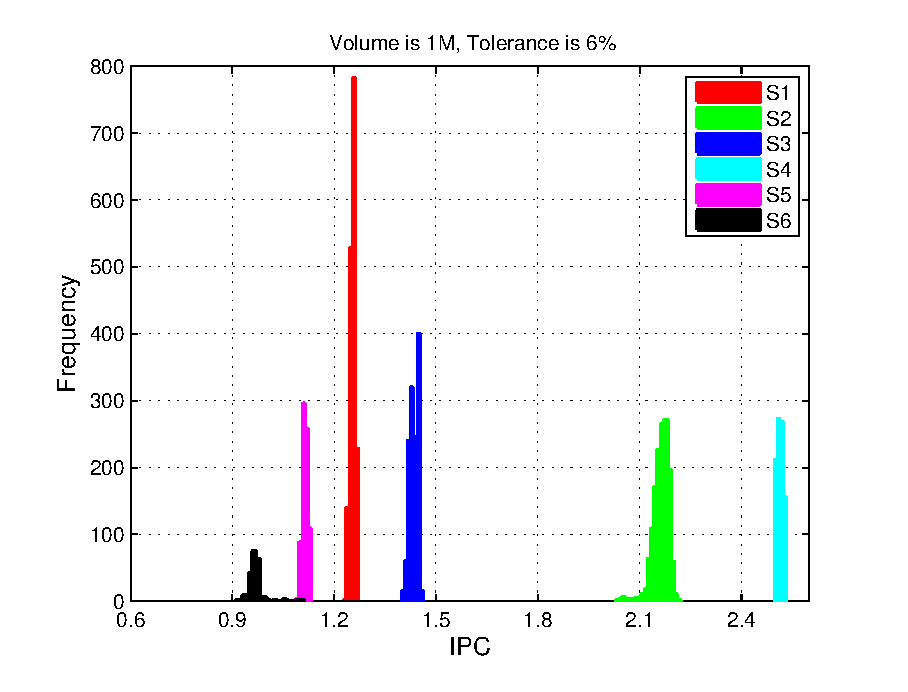
\includegraphics[width=0.45\textwidth]{SnippetDistributionlatest.eps}}
    \subfigure{\includegraphics[width=0.45\textwidth]{NewSnippetDeviationTolerance.eps}}
    \caption{Exemplifying the variation of six snippet classes (L) and the CDF of $10^3$ snippet classes (R)}
    \label{sdist}
\end{figure*}

\subsection{Dynamic Sick Core Ranking}
We take a new approach to characterizing the core-level performance. There are two unique perspectives that diverge from conventional performance measurements. 1) Rather than building dedicated benchmarks, we use the ordinary workloads as the benchmarks which are readily accessible in the field. 2) Rather than using the user visible system-level performance, we use microarchitectural-level operations (uops) to testify the core's performance. The rational is that the uop throughput of a core can more faithfully reflect the core's capacity, even though these uops may come from different applications. The uops statistics can be obtained by build-in performance counters.

We define a segment of uops as a "snippet" characterized by the frequency of different types of uops. For example, the snippet $s=[fmul:60, fadd:35, branch:5]$ represents a 100-uop snippet comprised of 60 floating point (FP) multiply operations, 35 FP add operations, and 5 branch operations. A snippet servers as the basic micro-benchmark to testify a core's healthy condition. Many snippets constitute an epoch which corresponding to a OS scheduling interval. A workload is comprised of many epochs. The basic temporal granularity in CoreRank is shown in Figure \ref{granu}. Note that a valid snippet should not undergo the two types of stalls due to 1) uncore resources contentions, such as memory bandwidth, network congestions, and 2) threading synchronization, such as barriers, locks. These stalls can mislead the quantification of core healthy conditions because they are not caused by core defects.

In the following,  we first give an overview definition of healthy condition, and then describe how to use snippets to quantify it, followed by the validation of snippets. 

\subsubsection{Healthy Condition Definition}
The healthy condition ($H$) of core $i$ ($c_i$) is defined as a such metric that measures the degradation of core's performance ($P$) on snippet $m$ ($s_m$), $P(c_i|s_m)$, compared with a reference (degradation-free) core ($c_{ref}$), denoted by
\begin{equation}
  H(c_i|s_m) = \frac{P(c_i|s_m)}{P(c_{ref}|s_m)}.\label{hdef}
\end{equation}
Given healthy condition is reflected by the performance, we can directly use the performance as the proxy to healthy condition, that is
\begin{equation}
  H({c_i|s_m}) = {P(c_i|s_m)}, \label{healthy}
\end{equation}
where, $P(c_i|s_m)$ behaves like a random variable, but we find the randomness can be regulated well under properly defined snippets.

\begin{figure}[t]
  \centering
  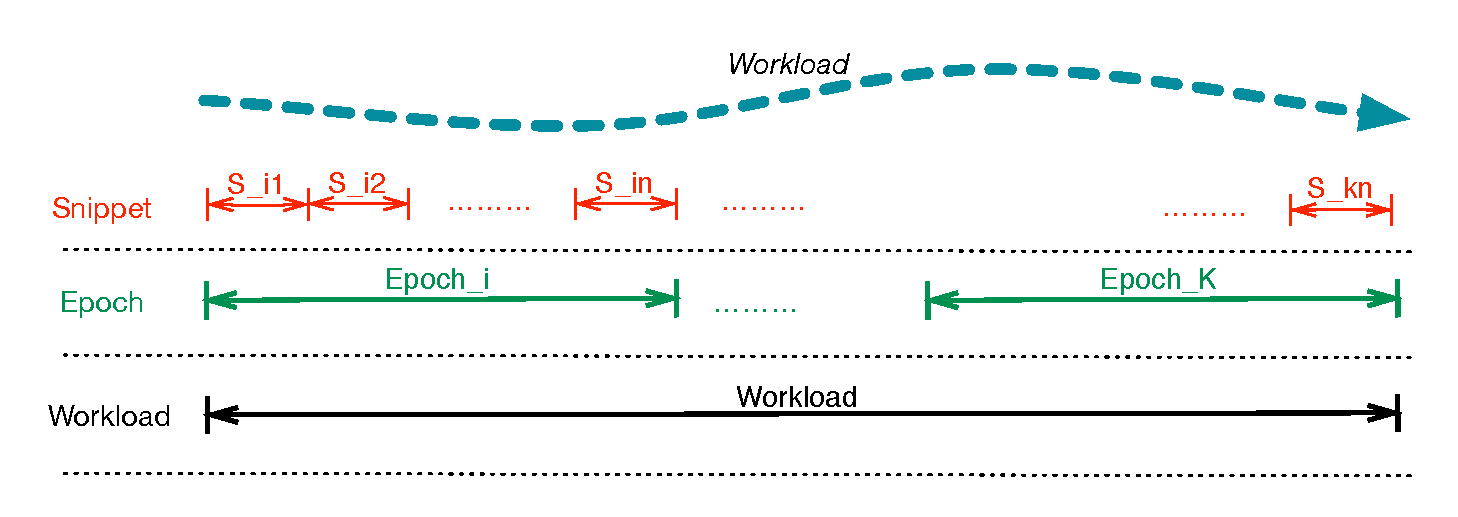
\includegraphics[width=0.7\textwidth]{granularity.eps}\\
  \caption{Temporal granularities of Snippet, Epoch, and Workload}\label{granu}
\end{figure}


\begin{figure*}[t]
\centering
\subfigure{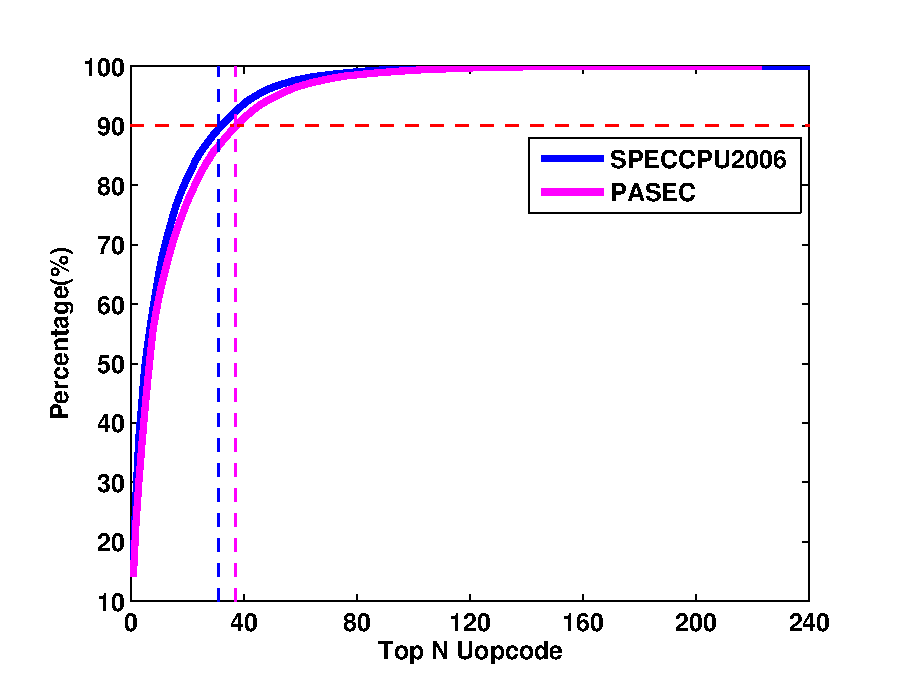
\includegraphics[width=0.45\textwidth]{InstructionActivities.eps}}
\subfigure{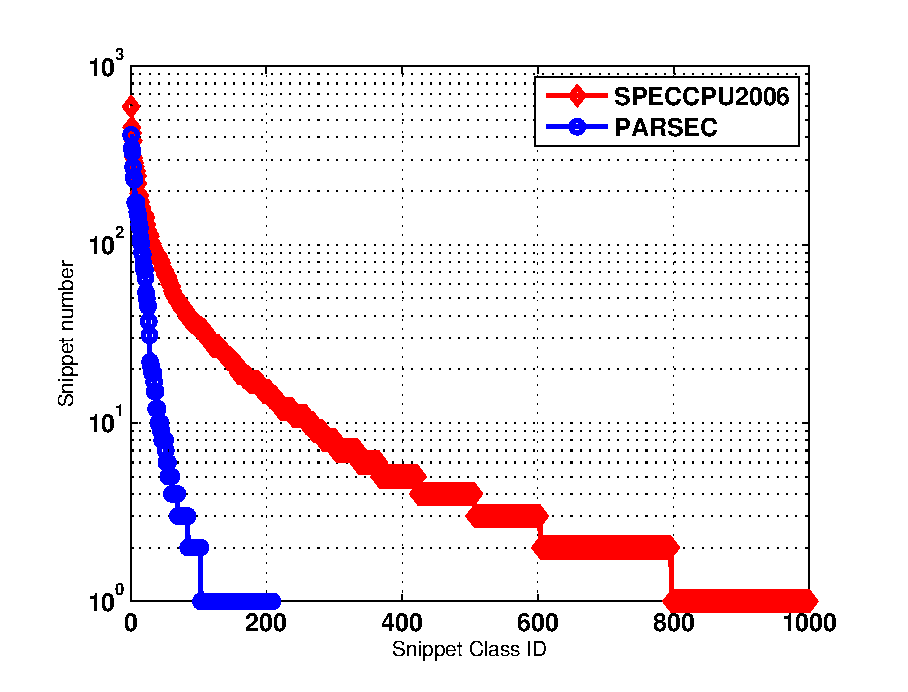
\includegraphics[width=0.45\textwidth]{SnippetSizeDistribution.eps}}
\caption{The uops frequency distribution (L)  and snippet occurrence  distribution (R)}
\label{hotdist}
\end{figure*}

\subsubsection{Snippet definition}
Snippet is used to characterize the dynamic streams of micro-operations; hence it is a microarchitecture-specific representation and aims to faithfully reflect the activity of various microarchitectural components.  Because a micro-operation is directly associated with the opcode of corresponding instruction (for complex instructions in CISC architectures, the micro-operation is referred to those decoded sub-instructions from the complex instructions), the snippet therefore is characterized by the combinations of various opcodes and associate frequencies.  Mathematically,  a snippet can be represented as the following vector:
\begin{equation}
 s=[op_{(1)}: f_{{(1)}}, op_{(2)}:f_{{(2)}}, \cdots, \\op_{(n)}:f_{{(n)}}],
\end{equation}
where  $op_{(i)}$ is the identification of the type $(i)$'s active micro-operation, and $f_{{(i)}}$ is the associate  frequency of occurrence.  


The definition of snippet holds two merits: 1) the popularity of different snippets exhibits prominently exponential distribution, which implies that we only need to study a set of ``basis" snippet to cover most operation streams in reality. 2) The degradations of the same snippet to the same core approximate to each other is context-insensitive,  which implies we can use the combination of basis snippets to calculate the performance impact of virtually any streams of uops.  Before delving into the detail validation, we first introduce three key attributes characterizing a valid snippet.

\begin{itemize}
    \item \textbf{Volume}: Snippet volume is defined as the total number of uops of the target snippet, i.e. $\sum_{i=1}^n f_{(i)} $. If two snippets, $s_1$ and $s_2$, are comprised of the same types of active operations and each type with the same frequencies, then we call the two snippets  belong to the same class $S$, denoted by $S=\{s_1, s_2\}$; otherwise they belong to different classes.

    \item \textbf{Capacity}: The number of snippets of a class, i.e. $|S|$, is defined as the class capacity. If we view $S$ as a random variable, then $s$ is actually a sample of $S$. Therefore, Eq. (\ref{healthy}) can be represented as
        \begin{equation}
            H(c_i|s_m)=P(c_i|S_m), \label{healthy2}
        \end{equation}
        where  $P(c_i|S_m)$ is the expectation performance of core $i$ on random variable $S_m$.

    \item \textbf{Tolerance}: In reality, we may relax the classification requirement by allowing a tolerance $\eta$ in frequency variations.  For example, $\eta=10\%$ means that the frequency of the same active uops with $\pm5\%$ variation can be viewed as equivalent.
\end{itemize}

\subsubsection{Snippet characterization}
In this section, we study the snippets performance distributions, population distribution, and the impacts of snippet volume and tolerance. 

\textbf{Snippet performance distribution is narrowly distributed.} Snippet classes can serve as ideal reagents to testify the healthy condition of cores because they are narrowly distributed, or called ``stable" in performance, no matter which application these snippets come from. As an example, we demonstrate the performance distribution of six snippet classes in Figure \ref{sdist}(L). The performance (measured by IPC) with volume of 10 million uops and tolerance of 6\%.   With such narrowly distribution, the mean value ($\mu$) of  $S$  on core $i$ can serve as a reasonable approximation to $P(c_i|S_m)$.

In fact, this merit of performance stability  is not a coincidence but  holds for majority of the snippet classes.  The stability can be reflected by the ratio of performance standard deviation and mean ($\sigma/\mu$).  The smaller  $\sigma/\mu$ implies higher performance stability.  We demonstrate stability of snippet classes with SPECCPU2006 and PARSEC benchmarks, which represent the multi-program and multi-thread workload, respectively. The result in Figure \ref{sdist}(R) shows that the $\sigma/\mu$ is no more than 5\% for more than 90\% snippet classes, when $\eta=6\%$.

Note that we do not emphasize that the distribution of $S$ has to be gaussian, even though it always tends to be as long as the \textbf{Capacity} is large enough. This trend is guaranteed by CLT (Central Limit Theorem).

\textbf{Exponential distribution of snippet population.} The reader may be wondering how many snippet classes, empirically, do the running applications have?   For example, for Intel Nehalem microarchitecture, there  are about 1125 types of uops, and the possible number of $S$ could be astronomical!   Fortunately, we find two exponential distributions can safely reduce the complexity, as shown in Figure \ref{hotdist}.

First, the "hot" uops usually are only small part of the whole number of uops. As Figure \ref{hotdist}(L) shows, the most frequently used top 80 uop types can cover over 97\% of uop streams.

Second, the "hot" snippet classes also are small part of the whole space. As Figure \ref{hotdist}(R) shows, the top 0.1 million snippets can be classified into about 50 and 200 classes for PARSEC and SPEC benchmarks, but more than 80\% classes contain a few snippets less than 10, compared to the top hot classes with thousands of snippets.  Hence, we can ignore those snippets classes with a small number of snippets.

\textbf{Impact of tolerance to performance stability.} To reinforce stable performance,  the tolerance plays a critical role. Generally, the tighter tolerance threshold, the higher performance stability, because tighter threshold leads to less frequency variation in each active uop. Figure \ref{tolerance} shows the $\sigma/\mu$ value at 90 percentile across a rang of tolerance. We can see the stability degrades roughly linearly with increasing tolerance threshold.

\begin{figure}[t]
  % Requires \usepackage{graphicx}
  \centering
  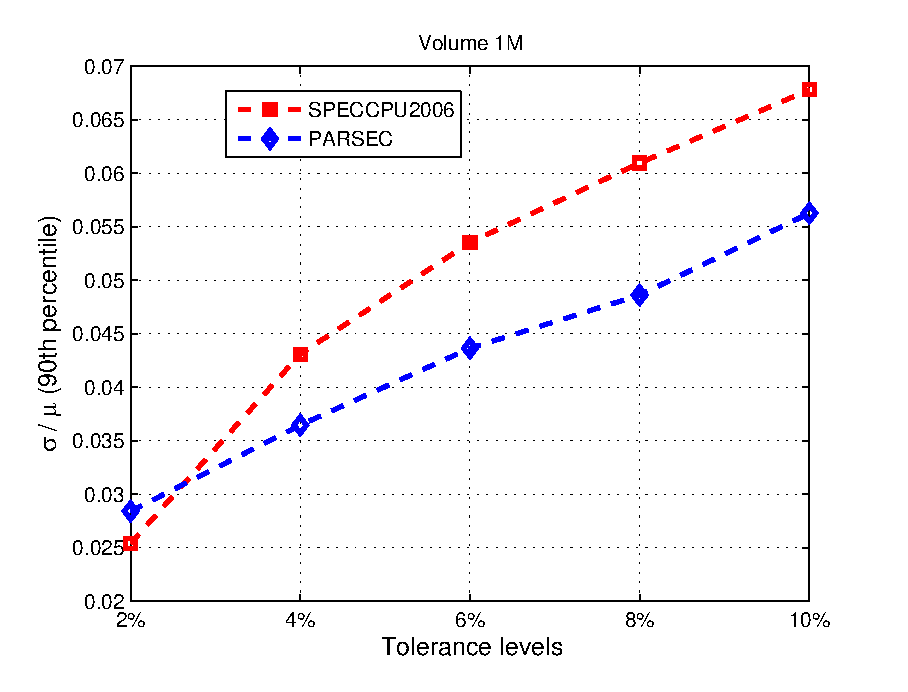
\includegraphics[width=0.65\textwidth]{NewSnippetDeviationToleranceVariation.eps}\\
  \caption{The impact of tolerance to stability}\label{tolerance}
\end{figure}


\textbf{Impact of volume.}
The volume size is a design tradeoff. If the volume is too large, then a snippet will experience high possibility to be invalid, due to uncore resources contentions or threading synchronization, but the overhead of snippet scheduling will be amortized well. However the volume smaller than the snippet scheduling interval is also unnecessary because the OS cannot exploit so fine-grained phase variations. Given the minimal Linux  scheduling time slice is 10ms \cite{PIE}, we set the volume to 10 millions of uops because its execution time is comparable to a time slice.


\subsubsection{Different snippets susceptible to different defects }
Clearly, different snippet classes may stress different core microarchitectural components. Hence, the healthy condition of cores will be snippet-specific, rather than conventional judgement "faulty" or "fault-free". Figure \ref{faultaware} clearly confirms this implication. As an example, we compare the performance of seven snippet classes on a fresh core (no degradation) against a degraded core (with half private L2 cache decoupled). The S2, S3, S4, and S6 shows to be resilient to this degradation, while S1 and S5 affected by this degradation. We call such phenomenon as snippet-specific healthy condition.

\begin{figure}[t]
  % Requires \usepackage{graphicx}
  \centering
  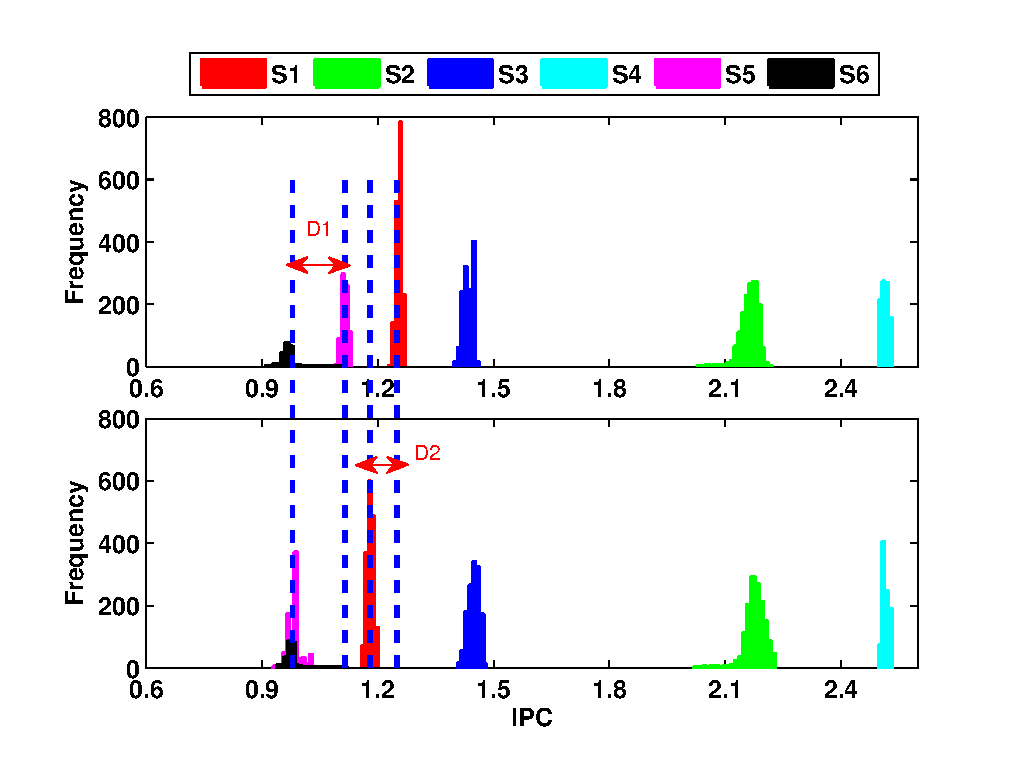
\includegraphics[width=0.7\textwidth]{NewSnippetFaultDeviationLatest.eps}\\
  \caption{Snippet-specific healthy condition}\label{faultaware}
\end{figure}


\subsubsection{Dynamic healthy condition quantification}
So far, we can obtain the healthy condition of any cores on any target $S$ by Eq. (\ref{healthy2}). These information can be logically organized into a matrix, denoted by $\mathcal{H}$
\begin{equation}
\mathcal{H}=\left[
\begin{array}{cccc}
H(c_1|S_1) & H(c_1|S_2) & \ldots & H(c_1|S_m)\\
H(c_2|S_1) & H(c_2|S_2) & \ldots & H(c_2|S_m)\\
\vdots & \vdots & \ddots & \vdots\\
H(c_n|S_1) & H(c_n|S_1) & \ldots & H(c_n|S_m)
\end{array} \right]
\end{equation}
where the element $H(c_i|S_j)$ represents the healthy condition of $c_i$ on $S_j$.

With the snippet-specific healthy condition, we can virtually calculate the healthy condition of a target core on any workloads. Suppose an epoch ($E$) of  a workload consists of $N_{S_i}$ snippets of class $S_i$, $i=1, 2, \cdots, m$, that is
\begin{equation}
E=[N_{S_1}, N_{S_2}, \cdots, N_{S_m}],
\end{equation}
then the healthy condition of  $c_i$ on $E$ can be calculated by
\begin{equation}\label{workloadperf}
  H(c_i|E) = \frac{\mathcal{H}(i, :)\times E^T}{\sum_{i=1}^{m}N_{S_i}},
\end{equation}
where $\mathcal{H}(i, :)$ is the $i$th row vector of $\mathcal{H}$; $E^T$ is the transpose of vector $E$. By characterizing the workload epoch by epoch, the OS is able to maximally hide the degradation of defective cores by judicious epoch scheduling between them. 

As a key intelligence of CoreRank, $\mathcal{H}$ is not static but dynamically refined to faithfully capture the cores' degradation.  $S_i$ $(i=1, \ldots, m)$ is dynamically updated by organizing the valid snippets in a FIFO (first in, first out) approach. We find that empirically using the capacity of 200 snippets  is a good choice to average out the small randomness, given $H(c_i|S_j)$ behaves as a random variable (even though with a narrow distribution).

\begin{figure}[t]
  \centering
  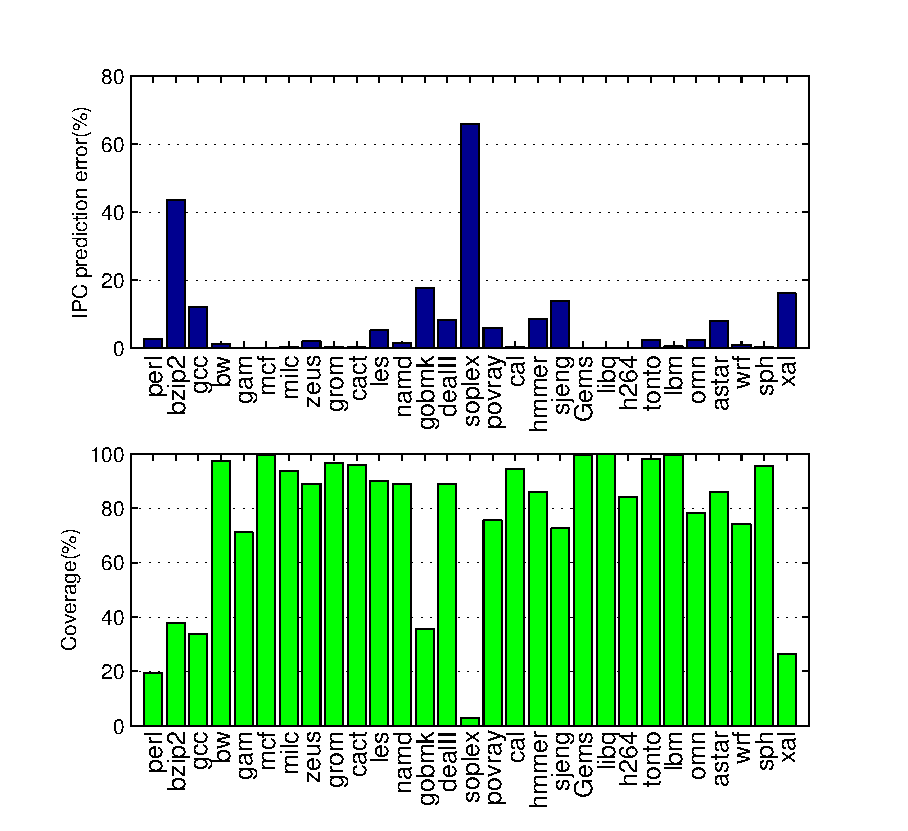
\includegraphics[width=0.75\textwidth]{IPCPredictionAndCoverage.eps}\\
  \caption{Validation of CoreRank in performance prediction accuracy (U) on a salvaged core with half L2 cache disabled, and corresponding workload coverage (L) by valid snippet classes.}\label{prederror}
\end{figure}


\subsubsection{Validation of healthy condition ($H$)}
In fact, according to definition, the healthy condition ($H$) can be interpreted as a kind of performance model measuring CPI (cycle per instruction).  To explicitly demonstrate the effectiveness of CoreRank model, we compare the performance obtained by CoreRank and the real performance on degraded cores. To make a fair comparison, we assume the threads wont be suspended or stalled, because, as explained in Section 3, those snippets undergo suspension/stalls are categorized as invalid micro-benchmarks and therefore cannot be used to testify the cores healthy conditions. The performance is translated to average IPC of a randomly chopped  phase with 1 billion instructions from SPEC CPU2006 benchmark suit. The error is defined as $\frac{ |IPC_{real}-IPC_{pred}|}{IPC_{real}}\times 100\%$, where $IPC_{real}$ is  measured value and $IPC_{pred}$ is obtained by CoreRank.  As shown in Figure \ref{prederror} (U),  the IPC prediction errors for most of the benchmarks are no more than 5\%.  Although the worst-case error reach up to unacceptable 60\% for \texttt{soplex}, such large error is not the limitation of CoreRank itself, but mainly because the the valid snippet classes cannot cover this workload due to insufficient snippets obtained in our experiment, as indicated in Figure \ref{prederror} (L).  The same reason also applies to other high-error workloads such as \texttt{bzip2}, \texttt{gobmk}, and \texttt{xal}. However, this is not a substantial limitation of CoreRank because in reality the coverage can very close to 100\% with sufficient snippet samples.  


\subsubsection{Impact of dynamic management}
According to the definition of healthy condition $H$, a core's $H$ is inferred from the statistics of sampled snippet performance. However, the actual performance,  measured in million instructions per second (MIPS) for example, may change because of engaging dynamic management for controlling thermal \cite{ThermalDVFS}, saving power \cite{PackCap}, or hiding aging effects\cite{ReviveNet}. An effective way to implement such dynamic management is through dynamic frequency (and corresponding voltage) adaptations (there is a large body of related references, just to name a few \cite{ReviveNet} \cite{ThermalDVFS}\cite{AgileRegulator}\cite{PackCap}).  

The actual core's performance, under dynamic  frequency scaling, may mislead the $H$ inference, since the low (high) performance may attribute to under-clock (over-clock) the core, rather than bad (good) healthy conditions. This problem can be solved by rectifying the performance statistics to a reference case.   Specifically, the original $H$ definition (Eq. (\ref{hdef}) ) is revised to
\begin{equation}
  H(c_i|s_m) = \frac{P((c_i, f_{act})|s_m)}{P((c_{ref}, f_{ref})|s_m)} =  \frac{P(c_i|s_m)}{P(c_{ref}|s_m)} \times \eta,
\end{equation}
where $\eta$ is the performance speedup attributing to frequency tuning from $f_{ref}$ to $f_{act}$. It can be obtained by online \cite{AgileRegulator}  or offline regressions.   The most naive $\eta$ can be approximated by  $ f_{ref} /f_{act}$ (more sophisticated $\eta$ can provide more accurate inference; the detail is beyond the scope of this paper).  By incorporating parameter $\eta$,  the framework of CoreRank can be applied to systems with dynamic management.  


\subsubsection{Handling failed cores}
Even though this paper focuses on the core progressive degradation, i.e. the cores still functionally work in the presence of salvageable defects in field \cite{salvaging}. Dealing with failed cores, or "dead" cores,  is relatively easy by simply disabling them, i.e. all elements of the corresponding row vector of $\mathcal{H}$ are set to "0". The core salvaging can be implemented by exploiting the natural microarchitectural redundancy. The technical details of diagnosis \cite{diagnosis}\cite{trace-based-diagnosis}\cite{mswat} and salvaging \cite{salvaging}\cite{exploiting-redundancy} are beyond the scope of this paper.

\begin{figure*}[t]
  % Requires \usepackage{graphicx}
  \centering
  \includegraphics[width=0.95\textwidth]{imple2.eps}\\
  \caption{CoreRank implementation}\label{flow}
\end{figure*}

\subsection{Core Ranking Implementation}
CoreRank works like a high frequency sampling system. A software-implemented version can cause performance overhead  if the snippet volume is small. Suppose snippets with one million uops volume are encoded with 256 bytes, then the estimated sample frequency is about 2KHz at 1GHz core frequency and two uops per cycle, which generates 512KB/s per core. For a processor with 100 active cores, the peak bandwidth to move out these sample data can reach up to 50MB/s, even without considering the performance counter reading overhead which will burden the IO bandwidth. But a software-implementation is possible when taking larger snippet volume on manycores with small core counts.

In this paper we propose a hardware-implemented version which provides the OS core healthy information to make better resource management.  The only modification to current performance counter scheme is to log the opcode information, and build a hash table with hundreds of buckets storing the information of $\mathcal{H}$. To minimized the hardware overhead, we design a Time Division Multiplexer (TDM) style CoreRank, as shown in Figure \ref{mux}, where each CoreRank handles 16 cores.  This TDM hardware optimization exploits the fact that the process of quantifying healthy condition is timing non-critical.

\begin{figure}[t]
  % Requires \usepackage{graphicx}
  \centering
  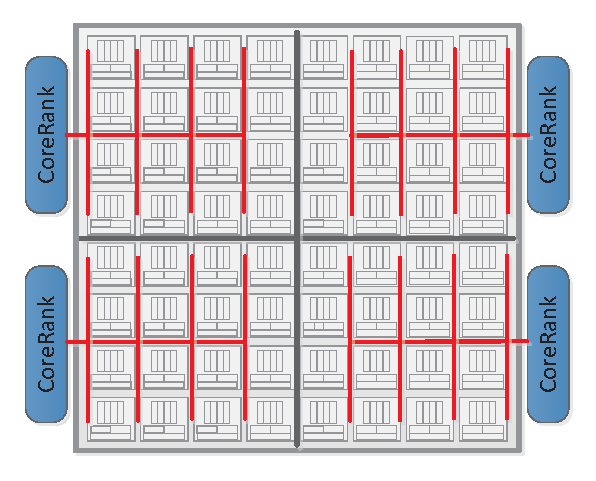
\includegraphics[width=0.6\textwidth]{mux1.eps}\\
  \caption{Time Division Multiplexer (TDM) style CoreRank to reduce the hardware overhead}\label{mux}
\end{figure}

The basic CoreRank mechanism can be divided into four steps, as shown in Figure \ref{flow}(a). First, we sample the uops streams with a set of performance counters which log the uops types and associated frequency, and clock cycles. These data is encapsulated as snippets.  Then, these snippets are classified to build snippet classes $S$. Because a qualified $S$ should possess small deviations, so we make a deviation test in step three. The $S$ passed the deviation test is qualified to update the healthy matrix $\mathcal{H}$.  Among the four steps, the classification is the most complicated in hardware implementation.  Traditionally, the classification is computationally difficult (NP-hard). We develop a novel efficient classification approach, detailed as follows.

\subsubsection{Classification}
When a new snippet is collected, we first regularize it by filtering those ``minority" uops whose frequency percentages are smaller than a predefined threshold, 0.5\% of the volume for example. These minority uops have little impact on the overall performance, but can greatly complicate the classification. By doing so, the dimension of snippets can be significantly reduced.

The classification allows a tolerance in frequency variation, which can be easily implemented by ignoring the least-significant bits in frequency of each type of uops.  The main decision-making process is shown in Figure \ref{flow}(b). We use a bloom filter to quickly decide whether this snippet belongs to an already existing snippet class $S$. If yes, this snippet goes through a hash table to find the associate classes and update it with the new sample. Otherwise, we cannot simply discard this snippet, but have to carefully decide whether this snippet belongs to a new class that has not existed so far. Our solution is to build a dummy class $S'$ for this snippet, and then enable a decay timer. A dummy class will be allowed to change into a qualified class as long as its capacity can reach a threshold in one counting period of the decay timer; otherwise, this snippet and associate dummy class $S'$ can be safely discarded.

There are two key hardware components in the implementation: a Bloom filter and a Hash table. Bloom filter is a time-efficient and hardware-implemented friendly  structure used to test whether an element ($s$) is a member of a set ($S$).  The basic principle can be explained with Figure \ref{bfilter} which illustrates a bloom filter with $m$-bit signature vector and $n$ hash functions. If a snippet $s$ has been proven not a minority, then, the bloom filter needs to be updated: the $n$ hash functions map the $s$ into $n$-bit of the signature vector and set the corresponding bit into 1. In filter mode, if the $n$-bit signature of a new snippet $s$ has been set in the signature vector, called a ``hit" in the bloom filter, this $s$ belongs to a qualified $S$; otherwise called a ``miss".

\begin{figure}[t]
  % Requires \usepackage{graphicx}
  \centering
  \includegraphics[width=0.65\textwidth]{bloomfilter2.eps}\\

  \caption{Bloom filter in snippet classification}\label{bfilter}

\end{figure}

\subsubsection{Deciding design parameters}
Bloom filter \cite{bloomfilter} has a good merit of no false negative, but may suffers from false positive, i.e. erroneously claim that $s$ belongs to a class $S$.  The probability of false positive  is given as  $P_{fp}=(1-e^{-nk/m})^n$, $k$ is the number of classes successfully mapped into the $m$-bit signature vector.  The optimal number of hash functions can be calculated by
\begin{equation}
  n=\lceil \frac{m}{k}ln2\rceil.
\end{equation}
We can see from Figure \ref{hotdist}(b),  empirically setting $k$ to 400 should be enough, then $P_{fp}$ and optimal $n$ would be functions of $m$, as shown in Figure \ref{evalubf}. The result shows that a bloom filter configured with at least 5000-bit signature vector and 9 hash functions can keep the false positive rate below 0.5\%, and therefore is a recommend design point.  In implementation, we use a 8192-bit ($2^{13}$) signature vector and 10 hash functions.

The snippet classes are managed with a hash table, as Figure \ref{hashtable} exemplifies. The set of uops types and associated frequency of a $S$ serve as the key. Each class is associated with a bucket storing the corresponding IPC of each snippet in that class.  The bucket is organized as a FIFO buffer to capture the most up-to-date core degradation degree.

\begin{figure}[t]
  % Requires \usepackage{graphicx}
  \centering
  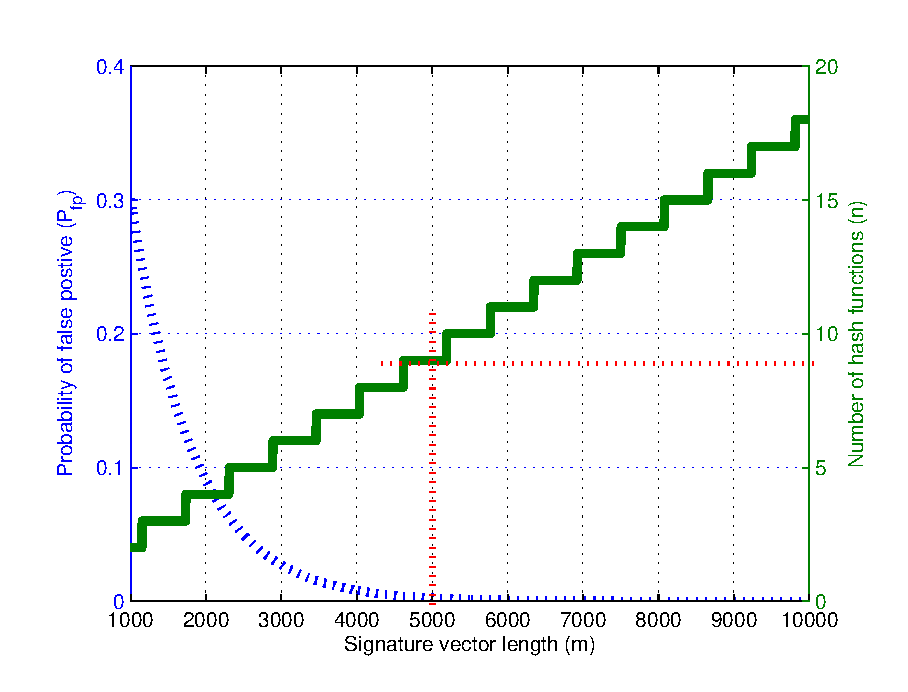
\includegraphics[width=0.65\textwidth]{evalu_bf.eps}\\
  \caption{Bloom filter design space}\label{evalubf}

\end{figure}

\begin{figure}[t]
  % Requires \usepackage{graphicx}
  \centering
  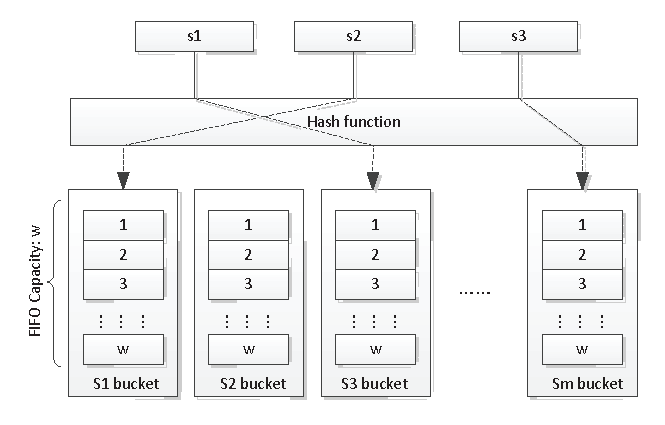
\includegraphics[width=0.75\textwidth]{hashtable2.eps}\\
  \caption{Hash table}\label{hashtable}
\end{figure}

\subsubsection{Choosing appropriate hash functions}
We have two types of hash functions, one for the 8192-bit bloom filter, and another for a hash table. The bloom filter uses MD5 \cite{md5} as the hash function. MD5 is a powerful hash function producing a 128-bit hash value. We divide the 128-bit hash value into 10 13-bit sub-hash values (the right-most sub-hash is padded with two ``0" bits)   to set corresponding bits in signature vector; each sub-hash value behaves as a different hash function mapping to individual location in the 8192-bit signature vector.

However, managing the snippet classes is more tricky. We find it requires very low, even not zero, collision rate because a snippet class polluted by other snippets out of that class is probably rejected by the deviation test. Hence, a perfect hash is virtually necessary. However, we find it's hard to design any even close-to-perfect hash function resulting in negligible collision rate. We have testify three types of hash functions, Segment Hash (i.e. split the original keys into segments, then map each segment to an integer, and finally combine the integers to map to a bucket.), Pearson Hash \cite{pearsonhash}, and Modulo Hash \cite{modulo}, but none performs good enough. As Figure \ref{hashresult} shows, even we map the classes into a 1024-bucket hash table, the collision rate is still as high as 10\%.

Therefore, we use direct map approach to achieve the effect of perfect hash. The detail is using the MD5 signature to directly tag each bucket.  When encounter a new class, we assign a free bucket to the new class and tag the bucket with its MD5 signature. The MD5 signatures have no collisions, so does the corresponding bucket assignments.  The overhead is the search complexity. However, the complexity is affordable because we only need to manage several hundreds of buckets and it is no more complex than indexing a cache with comparable number of cache blocks.

\begin{figure}[t]
  % Requires \usepackage{graphicx}
  \centering
  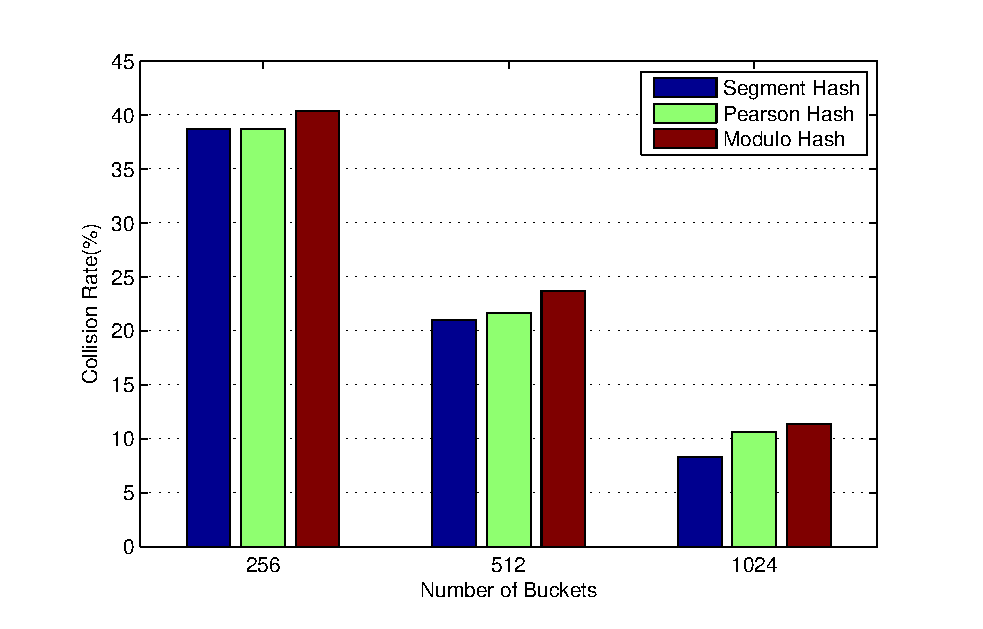
\includegraphics[width=0.6\textwidth]{Result_Hash.eps}\\
  \caption{Collision rate of different hash functions}\label{hashresult}
\end{figure}


\subsubsection{Handling sparsity of $\mathcal{H}$}
The healthy matrix $\mathcal{H}$ is progressively built and updated.  So, some elements of $\mathcal{H}$ may be unavailable until the  qualified snippet classes are obtained from the corresponding cores. We use a ``default-first" policy to assign the default value to those unavailable elements.  According to this policy,  the unavailable elements are assigned positive infinite value ($+\infty$), which implies the healthy condition is so well that the cores tend to be activated to work immediately.  This policy is helpful to quickly explore the cores and reduce the sparsity as soon as possible.

\subsubsection{Hardware overhead}
The main hardware overhead comes from the bloom filters and MD5 hash function. From Figure \ref{hotdist}(b), we can figure out a 512-bucket hash table should be enough. The detailed overhead includes hash functions, bloom filters, MD5 registers, and some associative search logics. We implemented the CoreRank logic into RTL with verilog, and synthesized it with Altera Quartus tool. The overhead is shown in Table \ref{overhead}. The results show that a CoreRank imposes about 1.7M logic gates and 21KB storage. This overhead is small compared to a processor with  billion transistors.   Furthermore, with TDM mechanism, the overhead can be further amortized.

\begin{table}[t!]
\caption{CoreRank hardware overhead}\label{overhead}
\begin{center}\small
\vspace{0.2cm}
\scalebox{1}[1]{
\begin{tabular}{|l|c|c|}
\hline
 \textbf{Component}   &   \textbf{Comb. logic gates (K)} &\textbf{Storage(KB)}\\
\hline
\hline
MD5                     &76      &       0.1       \\
\hline
 Bloom filter    &  1582   &   12.6       \\
\hline
Pearson Hash  & 0.62 & 0.6  \\
\hline
Bucket                &   0.38 & 7.3    \\
\hline
Others                 &   61.2   & 0.2 \\
\hline
Total                   &1720  &   20.8   \\

\hline
\end{tabular}}

\end{center}
\end{table}

\begin{figure*}[t]

 \centering
  \includegraphics[width=0.8\textwidth]{MediumDegradationWithAndWithoutCoreRank41.eps}\\
\caption{Performance comparison between processors without (L) and with CoreRank (R)}
\label{comp1}
\end{figure*}

\subsection{Experiment Result Analysis} \label{sec:3}
\subsubsection{Experimental Setup}
We evaluate CoreRank scheme with Sniper \cite{sniper}, a multi-core simulator based on the interval core model\cite{IntervalSimulation} and Graphite\cite{Graphite} simulation infrastructure. Sniper can accurately simulate x86 architecture at a speed of serval MIPS (million instructions per second). Sniper uses Intel Pin tool (version 61147) to dynamically profile the stream of uops of each cores, which provides us a easy way to collect snippets in the experiments.   We use a 12x12 manycore as the baseline to evaluate the performance.

We run through SPECCPU2006 and PARSEC benchmark suits, which generates over ten thousands of snippets under different core degradation models. We assume each core, if has defect,  only suffers from a single type of defects to make the time-consuming experiment affordable.   We configure the core  according to Intel Nehalem microarchitecture which has 1125 types of uops.  Table \ref{Exp} shows the basic core configuration.   In terms of snippet, otherwise specified, the snippet volume is 10M, the capacity of each snippet class is 200, with tolerance of 6\%.


\begin{table}
\caption{Core configuration}\label{Exp}
\begin{center}\small
    \begin{tabular}{|l|c|}
  \hline
  \textbf{Parameter} &\textbf{ Value} \\
  \hline
  \hline
  Frequency & 1GHz \\
  \hline
  L1 I/D cache 32KB &  Cache line 64B, associativity 4 \\
 \hline
  L2 cache  512KB &  Cache line 64B, associativity 8 \\
  \hline
  Issue Width &  4 \\
  \hline
  Branch predict entry  &  1024\\
  \hline
  Instruction Window &  96 \\
  \hline
  \end{tabular}
  
  \end{center}
\end{table}

\subsubsection{Workloads}
We  build two types of workloads: SPEC CPU2006 for multi-program workloads, and PARSEC to multi-thread workloads.  The manycore is always fully loaded with the synthesized workloads. For example, for multi-program workload, we randomly chose 12x12 benchmarks from the SPEC benchmark suite to feed the manycore.   For multi-thread workloads, we use 4-thread and 8-thread configurations, respectively.   Note that a specific benchmark can be repetitively chosen from the benchmark suites. To make diversity, each benchmark is fast-forward to different phases before sampling the snippets.


\textbf{Application mapping policy:} To demonstrate the application of CoreRank, we have to fairly compare the performance between processors with and without CoreRank.  The performance is measured by summing up all of the active core IPC within the same time window. When measuring the performance degradation, we use the geometric mean of slowdown of all cores.  For processor without CoreRank, it's reasonable to assume that applications are randomly mapped to the cores with different degradations, since we have no way to distinguish which core is superior to another. By contrast, for that with CoreRank, we assume a policy that maximizes the overall performance. This can be achieved by using Eq. (\ref{workloadperf}). With this equation, we can figure out  which core is the best for a given workload. For experiment, we assume $w$ can be predefined by a perfect profiling. But in reality, $w$ should be dynamically predicted. In addition, when comparing the performance, we neglect the scheduling overhead because the execution time of a snippet is very comparable to a Linux OS time slice in reality.

\subsubsection{Result Analysis}
\begin{figure*}[t]
 \centering
  \includegraphics[width=1\textwidth]{Figure14DegradationLevelwithoutCoreRank41.eps}\\
\caption{Performance degradation on processors with mild(L), median(M), and severe(R) degradation models,  without CoreRank,  4-thread for multi-thread workloads.}
\label{comp2}
\end{figure*}

\begin{figure*}[t]
 \centering
  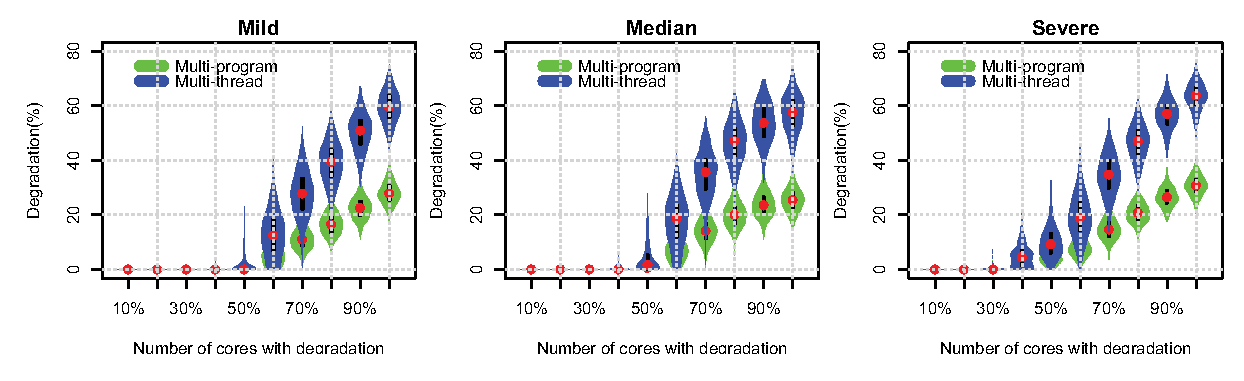
\includegraphics[width=1\textwidth]{Figure15DegradationLevelwithCoreRank31.eps}\\
\caption{Performance degradation on processors with mild(L), median(M), and severe(R) degradation models,  with CoreRank,  4-thread for multi-thread workloads.}
\label{comp3}
\end{figure*}

\textbf{Performance comparison:} First, we study the performance degradation with obliviousness to core healthy conditions.  Figure \ref{comp1}(L) shows the normalized performance degradation under gradually increased percentage of unhealthy cores.   The degradation model for each core is randomly chosen from the degradation models listed in Table \ref{degrademodel}, with ``median" degradation degree.  We run 500 workloads to highlight the statistical trend, presented by violin plot. \footnote{Violin plot is a statistical illustration of a group of values; the density of each value is reflect by the width on corresponding notch.}  

\textbf{The impact of unhealthy cores:} The result confirms the unhealthy cores can dramatically degrade the system performance.  Specifically, the multi-thread workloads are more sensitive than multi-program workloads to core degradations, because of  more prominent "cask-effect" in multi-thread workloads. The more thread-level parallelism, the more sensitive to core degradation. Also, we find the performance degradation goes relatively slowly, especially when the population of degraded cores exceeds 60\%, this is because  every multi-thread workload has  high possibility to be slowed down by at least one unhealthy core. Given the prevalent big-data processing today dominated by multi-thread programming model (MapReduce for example) and algorithms, the impact of unhealthy cores should not be underestimated.

The situation can be alleviated greatly with CoreRank, as Figure \ref{comp1}(R) shows. We assume an oracle scheduling policy, which directly uses CoreRank output to guide application mapping. The result shows that even the population of unhealthy cores is 50\%, the performance declines no more than 10\% even for the most susceptible 8-thread workloads, compared to the around 55\% degradation when oblivious to the cores' healthy conditions shown in Figure \ref{comp1}(L).  This is not surprising because the CoreRank can maximally hide the negative impact of unhealthy cores.

\textbf{The effectiveness of CoreRank:} CoreRank can successfully hide defects if the number of salvaged cores are less than 50\%. Comparing the Figure \ref{comp1}(L) and (R), we also conclude that it is  impractical to expect CoreRank helping revive a ``terribly sick" processor, i.e.  majority cores are salvaged.    As Figure \ref{comp1}(R) shows, when the unhealthy core population goes beyond 50\%, the performance degradation climbs quickly. The performance benefit is very slim  when the population of unhealthy cores crosses over 70\%.  Nevertheless, below 50\%, the processor, even with unhealthy cores,  can provide performance very close to a fresh one.

\textbf{An implication about processor retirement: } Since not all defective cores can be hidden, a key problem is when the unhealthy processor should be retired.  Based on the above result, we arrive at an interesting conclusion: the time when the salvaged cores take 50\% of a target processor probably can be used to define the lifetime of a manycore processors, because below this percentage the salvaged  cores can be hidden well.

\begin{figure*}[t]
 \centering
  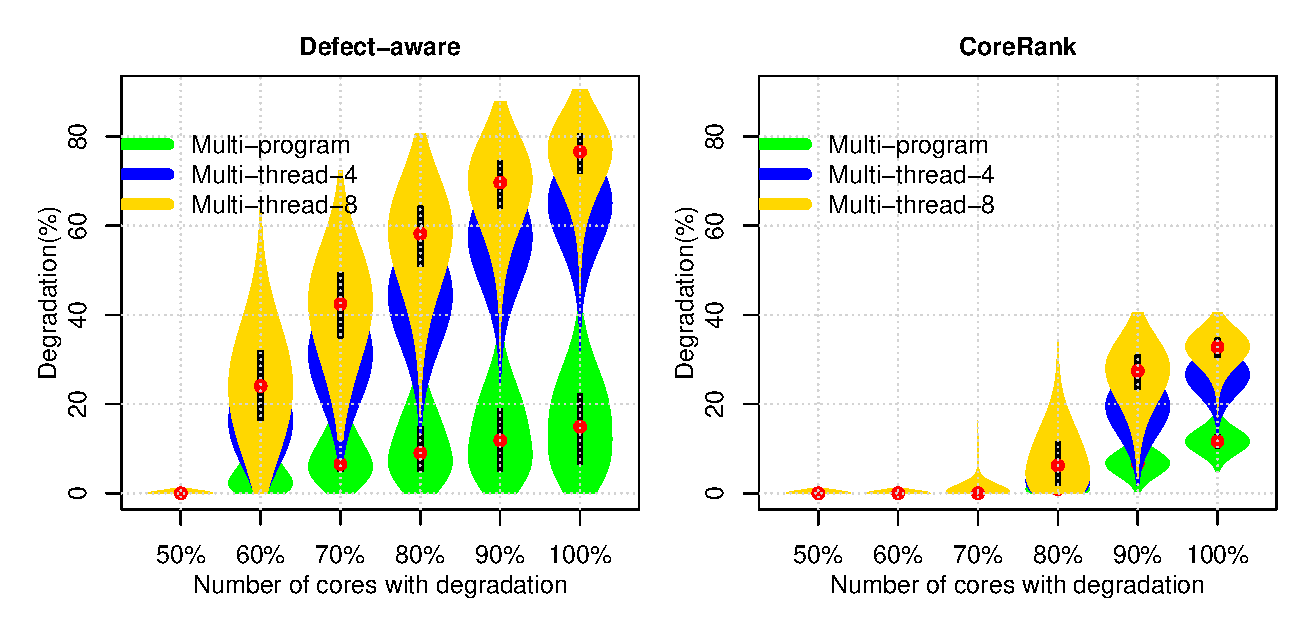
\includegraphics[width=0.8\textwidth]{Defect-awareCoreRank.eps}\\
\caption{Performance comparison between conventional Defect-aware scheme (L) and  CoreRank (R)}
\label{compdefectaware}
\end{figure*}

\textbf{Impact of various degradation degree:} The above results have studied the impact of median degradation degree. In this experiment we study how CoreRank responds to different degradation degrees. Figure \ref{comp2} shows the results of performance under \emph{mild}, \emph{median}, and \emph{severe} degradation, respectively.  Unexpectedly, we find the performance under mild and median shows very similar: the difference is merely 3$\backsim$5\% at each unhealthy populations. This is because most of the applications actually cannot fully exercise even the \emph{median} cores, so the \emph{mild} and \emph{median} make a little difference in performance.    But \emph{severe} causes more appreciable performance degradation.

An interesting difference emerges when we enable CoreRank.  Figure \ref{comp3} shows that even though all of the performance drops similarly to  that discussed in Figure \ref{comp1}(R),  the  takeoff points of degradation are different from each other.  The  severer degradation, the earlier appearance of the takeoff point.  For example, for \emph{mild}, the performance won't drop until around 50\% unhealthy cores reached. While for \emph{severe}, 30$\backsim$40\% unhealthy core can cause performance degradation.


\subsubsection{Comparing with defect-aware scheme}
To compare our scheme with a baseline that can be aware some defects by some means, we carefully set up another baseline, called Defect-aware, and a new set of experiments. We assume that a microprocessor has core-wise built-in fault-register which indicates which components suffer from defect during runtime. The OS, by reading these registers, is able to prioritize the degradation-free cores when mapping jobs.  In this comparison, the Defect-aware baseline follows the policy:  picks the defect-free cores first, then the cores with less degree of degradations, till all cores are put to use.  In this experiment, we assume the the core utilization is 50\%, i.e. only half of the cores are active.  The defective cores suffer random defects as listed in Table 1.  The results are shown in Figure \ref{compdefectaware}.  We can see if the defective cores take less than half of the core count, the Defect-aware scheme can always pop up the defect-free cores, so there will no performance degradation compared to the oracle case. However, with the increase of number of defective cores, the Defect-aware scheme cannot hide the defective cores well, even though it still prioritizes the core with mildest degradations.  By contrast, CoreRank shows to be more resilient to the escalating of defective cores by taking the workload-dependent characteristics.  

Note that, without CoreRank, Defect-aware baseline still has no ways to figure out which types of defects are more affectional to a given workload, i.e. Defect-aware baseline cannot quantify how different degradations affect the resultant performance, for various workloads. Take the degradation in issue width for example, Defect-Aware baseline can be aware the core with issue width degradation, so the job is better to be mapped to a defect-free core, or at least, to a core with less degree of issue degradation, if possible. However, as we know, the core with issue width defect shows to be resilient when running a workload with poor intrinsic IPC.  Therefore, assigning a thread with poor intrinsic IPC to such a core should not be much problematic. Such case-sensitive phenomena also happen to other microarchitectural components, such as cache, instruction window, and so on.  By doing so, we can save healthy cores for those threads more sensitive to certain types of defects.  In other words, it is not enough to only know whether a core suffers from what types of defects. 

CoreRank is designed to bride this gap. In CoreRank framework, it's more important to know how a defective core performs on a given workload, than to know which defect the core suffers from.  The former, i.e. the key idea of this article, focuses on how to make best use of the imperfect cores, while the later focuses on how to isolate the defects to ensure correctness (and has been intensively studied in the reliability community).   



\subsubsection{Comparing with heterogeneity-aware scheme}
CoreRank serves as a bottom mechanism to gain variability awareness.  Rangan et al. proposed an approach to maximize throughput in the presence of variation-induced heterogeneity in multi-core processors \cite{TDS}, where the heterogeneity refers to the various core frequencies. The key contribution is a scheduling algorithm, called Throughput-Driven Scheduling (TDS) targeting maximum chip throughput, which is in line with our objective to demonstrate the effectiveness of CoreRank.  

The difference from our approach is that TDS employes last-value predictor to serve as the fundamental mechanism to support epoch-by-epoch thread scheduling. TDS uses BIPS over a prediction period of 100K cycles  as the proxy of core performance level, and maps the applications, according to their computing intensities, to the cores with accordant performance levels; a more computing bounded application is assigned a core with higher performance level.   In our scheme, similar to cores with lower frequency due to process variation, the defective cores deliver lower performance, which serves as the ground for comparison. 

Figure \ref{compheteroaware} shows the comparison between TDS and CoreRank, on multi-program workloads.  Unsurprisingly, CoreRank outperforms TDS in hiding the the degradation. The key reason is that simply using the sampled BIPS to serves as the performance level, as TDS adopted,  is not alway reliable, because the BIPS is not only determined by the core itself, but also the threads executed. So, even the algorithm aims to maximize the throughput, but the sub-optimal scheduling is unavoidable due to unreliable core-level performance prediction.    


\begin{figure}[t]
 \centering
  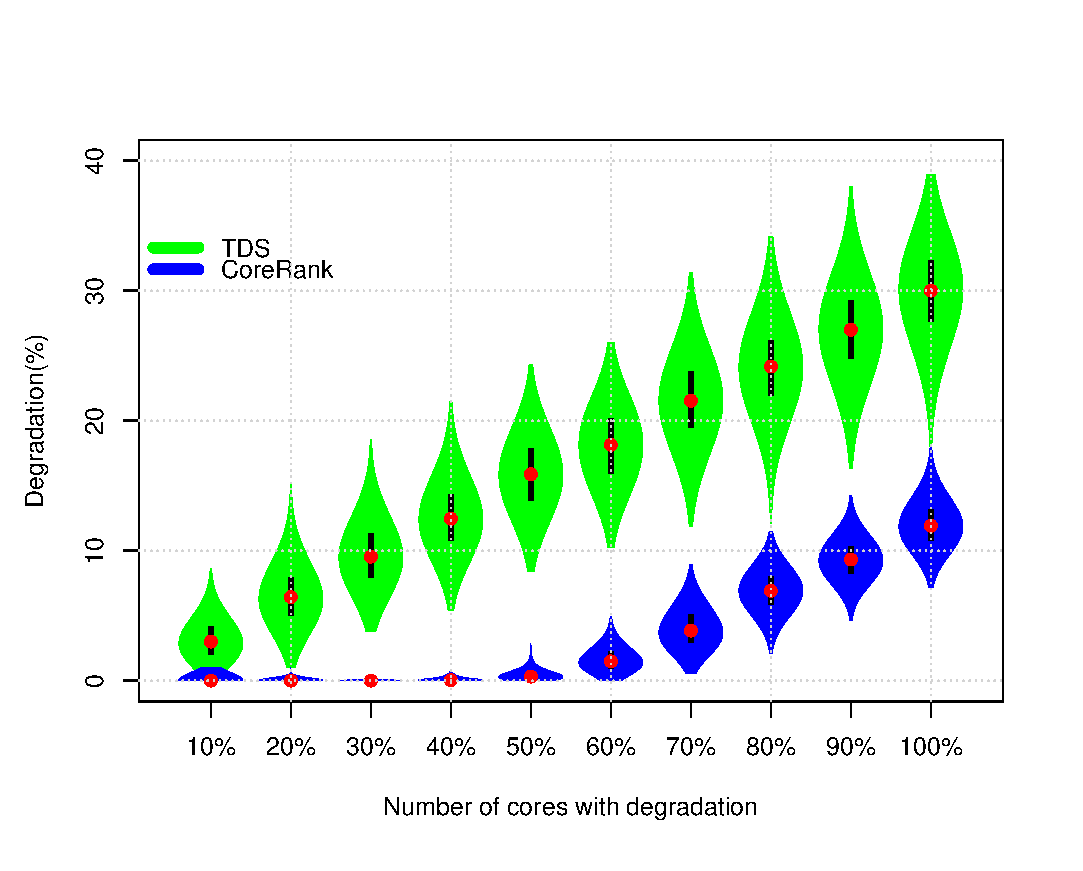
\includegraphics[width=0.75\textwidth]{fastCoreAndCoreRankComparision.eps}\\
\caption{Performance comparison between Throughput-Driven Scheduling (TDS) (L) and  CoreRank (R)}
\label{compheteroaware}
\end{figure}



%The core-to-core variation has been extensively studied. Many previous researches focus on the variation-aware optimization such as \cite{Variation_Aware_Application_Scheduling_isca08}\cite{dong_prdc09}\cite{mitigate} in terms of power, energy, performance, and reliability.  However, these researches assume the variation is constant and serves as a kind of input to their optimization procedures. The optimization algorithms may be also applicable to hide in the filed degradations, as long as the degradations can be clearly quantified on-the-fly. CoreRank is designed to provide such facility.

%Quantifying a processor performance is a key issue to compare various computer systems. The basic principle is by running a set of predefined benchmarks, such as SPEC CPU2006. Given the performance may change significantly on different benchmarks, and even the same benchmark on different runs, the prior work uses some statistical approaches, such as hypothesis test, to testify whether a computer is faster than another \cite{perfcomp}. This approach is valuable for computer evaluation, but hardly works for quantifying the in-flight core-level performance, because we have no means to reliably test an individual core of a manycore processor in service. CoreRank can solve this problem by sampling ``micro" benchmarks, i.e. snippets in this paper, to testify an individual core performance in a statistical way.

%The primary objective of core salvaging is to make a core with defects still functionally work, usually at degraded performance \cite{salvaging}\cite{Facelift_08}\cite{Duplication_05}\cite{exploiting-redundancy}. The defects may be resulted from imperfect manufacturing \cite{variation_jssc02}, or progressive transistor aging in the field \cite{DynamicNBTI_03}. With these sophisticated salvaging techniques, a manycore processor could ``live" longer, but with more prominent difference in core-to-core healthy conditions.  However, few prior researches focus on how to dynamically quantify such healthy variation. CoreRank aims to fill this gap and helps make better use of the salvaged cores with different healthy conditions.


\subsection{Discussion}
To be added.

\section{Summary}
Intermittent faults are emerging as a big challenge to reliable microprocessor design. In this paper,we propose a metric IVF to quantitatively characterize the vulnerability of microprocessor structures to intermittent faults. The IVF evaluation methodology contains the following aspects: 
\begin{itemize}
    \item analyze the physical causes of intermittent faults;
    \item classify intermittent faults into different fault models based on their behaviors;
    \item set key parameters for an intermittent fault and determine when the intermittent fault results in a visible error;
    \item for a specific microprocessor structure, propose IVF computation algorithms for different intermittent fault models;
    \item implement IVF computation algorithms in a high-level performance simulator, with which to compute IVF for the specific structure.
\end{itemize}

With the IVF evaluation methodology, we compute IVFs for reorder buffer and register file in terms of intermittent stuck-at faults, intermittent open and short faults, and intermittent timing faults. Experimental results show that intermittent stuck-at-1 faults have most serious adverse impact on program execution among these three types of intermittent faults. Besides, IVF varies noticeably across different microprocessor structures and program phases. Our experimental results imply partial protection of the most vulnerable structures and program phases to enhance system reliability. With the guide of IVF evaluation methodology, we also discuss several possible intermittent fault detection and recovery techniques which can be used to improve system reliability.

Quantifying the performance response of cores with degradation is a fundamental problem to make best use of the manycore processors suffered from ``sick silicon". In this paper, we find that the core performance depends on not only applications, but also specific hardware components with degradation. We therefore develop a new metric, healthy condition, to capture this implication. Then, we propose CoreRank to quantify the core-level healthy condition. CoreRank samples the uops streams to build micro-benchmarks, called snippets,  to testify  cores with different degradation. We also propose a detailed implementation of CoreRank. Experimental results show that with CoreRank, the performance degradation of a manycore can be reduced significantly. We believe that CoreRank is instructive to other dynamic performance optimizations for future large-scale manycore processors.

\bibliographystyle{plain}
\bibliography{refs}


